% **************************************************
% Macro specifiche per il documento corrente
% **************************************************
% Nome
\newcommand{\docName}{Piano di Qualifica}
% Nome file
\newcommand{\docFileName}{piano\_di\_qualifica.3.0.pdf}
% Versione
\newcommand{\docVers}{3.0}
% Data creazione
\newcommand{\creationDate}{2012-12-10}
% Data ultima modifica
\newcommand{\modificationDate}{2013-03-16}
% Stato in {Approvato, Non approvato}
\newcommand{\docState}{Approvato}
% Uso in {Interno, Esterno}
\newcommand{\docUsage}{Esterno}
% Destinatari da specificare come nome1\\ &nome2\\ ecc.
\newcommand{\docDistributionList}{Prof. Tullio Vardanega\\ & Prof. Riccardo Cardin \\& Dott. Gregorio Piccoli}
% Redattori da specificare come nome1\\ &nome2\\ ecc.
\newcommand{\docAuthors}{Andrea Rizzi\\&Stefano Farronato\\ &Elena Zecchinato}
% Approvato da
\newcommand{\approvedBy}{Diego Beraldin}
% Verificatori
\newcommand{\verifiedBy}{Riccardo Tresoldi}
% Perscorso (relativo o assoluto) che punta alla directory contenente shared/
% come sua sottodirectory (per comodità chiamiamola 'doc root').
\newcommand{\docRoot}{..}
% definire se si vuole l'indice delle tabelle
\def\INDICETABELLE{false}
% definire se si vuole l'indice delle figure
\def\INDICEFIGURE{false}

% importa il preambolo condiviso da tutti i documenti
% shared/preamble.tex
%
% Questo documento contiene la parte del preambolo condivisa e viene pertanto
% richiamato nel 'master' di tutti i documenti di progetto.  Al suo interno
% contiene le inclusioni (e le configurazioni) di tutti i package richiesti per
% la compilazione dei documenti, le macro di carattere generale e la definizione
% degli stili di pagina.

\documentclass[a4paper,10pt,openright]{article}

% **************************************************
% Macro generiche
% **************************************************
\newcommand{\team}{Software Synthesis}                    % chi siamo
\newcommand{\email}{software.synthesis@gmail.com}         % e-mail
\newcommand{\caName}{}                                    % titolo capitolato
\newcommand{\caDescr}{}                                   % descrizione
\newcommand{\inglese}[1]{\textit{#1}}

% **************************************************
% Codifica e lingua dei documenti
% **************************************************
\usepackage[utf8x]{inputenc}                              % codifica caratteri dei documenti sorgenti
\usepackage[english,italian]{babel}                       % localizzazione ai fini di sillabazione e cross-references
\usepackage[T1]{fontenc}                                  % codifica font di output

% **************************************************
% Definizione geometria della pagina
% **************************************************
\usepackage[a4paper,head=4cm,top=4.5cm,bottom=3cm,left=3cm,right=3cm,bindingoffset=5mm]{geometry}

% *************************************************
% Intestazioni e piè di pagina personalizzati
% *************************************************
\usepackage{fancyhdr}
% stile normale
\fancypagestyle{normal}{
\fancyhead{}                                              % intestazione
\fancyhead[RE,RO]{
\begin{picture}(0,0)
  \put(-410,0){
\includegraphics[width=1.02\textwidth]{header_logo}}
  \put(-410,10){\sffamily\large\leftmark}
\end{picture}
\vspace{-4pt}
}
\renewcommand{\headrulewidth}{.4pt}                       % riga sotto l'intestazione
\cfoot{}                                                  % piè di pagina
\fancyfoot[RO,LE]{\sffamily
  pag.~\thepage{} di \pageref{LastPage}}                  % a dx nelle pag. dispari e a sx in quelle pari
\fancyfoot[RE,LO]{\sffamily\docFileName{} -- v.\docVers}
\renewcommand{\footrulewidth}{.4pt}                       % riga sopra il piè di pagina
}
% stile per gli indici
\fancypagestyle{toc}{
\fancyhead{}                                              % intestazione
\fancyhead[RE,RO]{
\begin{picture}(0,0)
  \put(-410,0){
\includegraphics[width=1.02\textwidth]{header_logo}}
\end{picture}
}
\renewcommand{\headrule}{}                                % nessuna riga sotto l'intestazione
\cfoot{}                                                  % piè di pagina
\fancyfoot[RO,LE]{\sffamily\thepage{}}                    % a dx nelle pag. dispari e a sx in quelle pari
\fancyfoot[RE,LO]{\sffamily\docFileName{} -- v.\docVers}
\renewcommand{\footrulewidth}{.4pt}                       % riga sopra il piè di pagina
}

\pagestyle{fancy}                                         % premetto: non so usare bene le marche:
\renewcommand{\sectionmark}[1]{\markboth{#1}{#1}}         % se qualcuno ha idee migliori si faccia avanti!

% **************************************************
% Tabelle
% **************************************************
\usepackage{tabularx}                                     % tabelle di larghezza fissa con una o più colonne variabili
\usepackage{multirow}                                     % colonne con colonne che si estendono per più righe
\usepackage{booktabs}                                     % per inserire l'ambiente table e le righe orizz. nelle tabelle
\usepackage{longtable}			                          % tabelle oltre i limiti di pagina

% **************************************************
% Cross-references e collegamenti ipertestuali
% **************************************************
\usepackage[hidelinks]{hyperref}
\hypersetup{%
  colorlinks=false, linktocpage=false, pdfborder={0,0,0}, pdfstartpage=3, pdfstartview=FitV,%
  urlcolor=Cyan, linkcolor=Cyan, citecolor=Black, %pagecolor=Black,%
  pdftitle={\docName}, pdfauthor={\team}, pdfsubject={}, pdfkeywords={},%
  pdfcreator={pdflatex}, pdfproducer={pdflatex with hyperref package}%
}

% **************************************************
% Immagini e grafica
% **************************************************
\usepackage{graphicx}                                     % supporto ad aspetti avanzati delle immagini
\graphicspath{{\docRoot/pics/}}                           % percorso contenente tutti i file immagini
\usepackage{color}                                        % permette di colorare facilmente il testo

% **************************************************
% Altri pacchetti opzionali
% **************************************************     
\usepackage{lastpage}                                     % per sapere il numero totale di pagine
\usepackage{lipsum}                                       % genera "dummy text" per prove di impaginazione
\usepackage{eurosym}                                      % per il simbolo dell'euro usare \EUR{x} dove x è l'importo



\renewcommand{\appendixname}{Appendici}

% Fine del preambolo e inizio del documento
\begin{document}

% Inclusione della prima pagina
% shared/firstpage.tex
%
% Questo documento definisce il contenuto della prima pagina, che si suppone
% essere uguale in tutti i documenti.  Oltre al logo e al titolo, la prima
% pagina contiene i metadati relativi al documento in cui viene inclusa.


% rimuove intestazioni e piè di pagina
\pagestyle{empty}

\begin{center}

% logo del gruppo

\includegraphics[width=1.5\textwidth]{logo}

\vspace{1in}

% titolo del documento
{\Huge\bfseries \docName}

\vspace{1in}

% tabella riepilogativa
\begin{tabularx}{.7\textwidth}{>{\bfseries\sffamily}l>{\sffamily}l}
\toprule
\multicolumn{2}{>{\sffamily}c}{Informazioni sul documento}\\
\midrule
Nome file:            & \docFileName\\
Versione:             & \docVers\\
Data creazione:       & \creationDate\\
Data ultima modifica: & \modificationDate\\
Stato:                & \docState\\
Uso:                  & \docUsage\\
Redattori:            & \docAuthors\\
Approvato da:         & \approvedBy\\
Verificatori:         & \verifiedBy\\
\bottomrule
\end{tabularx}

\end{center}

\newpage


% Storico delle modifiche
\section*{Storia delle modifiche}
\begin{longtable}{lp{.3\textwidth}lll}
\toprule
Versione & Descrizione intervento & Redattore & Ruolo & Data\\
\midrule % inserire qui il contenuto della tabella

3.0 & Approvazione documento& Diego Beraldin &Responsabile & 2013-03-16\\
2.8 & Correzione errori riscontrati in fase di verifica& Stefano Farronato &Progettista & 2013-03-16\\
2.8 & Verifica lessico ortografica del documenti& Riccardo Tresoldi &Progettista & 2013-02-16\\
2.7 & Aggiornata sezione ``Dettaglio dell'esito delle revisioni'' e ``Appendice'' & Elena Zecchinato &Progettista & 2013-03-16\\
2.6 & Aggiornata sezione ``Dettaglio dell'esito delle revisioni'' e ``Appendice'' & Elena Zecchinato &Progettista & 2013-03-15\\
2.5 & Aggiunta sezione ``Autovalutazione'' & Andrea Rizzi &Progettista & 2013-03-15\\
2.4 & Aggiornate e corrette definizioni analisi statica e dinamica & Stefano Farronato &Progettista  & 2013-03-15\\
2.3 & Riscritta sottosezione ``Metriche''  & Stefano Farronato &Progettista  & 2013-03-14\\
2.2 & Corretta sezione ``Metriche e metodi'' in ``Tecniche, metodi e metriche'' & Elena Zecchinato &Progettista & 2013-03-14\\
2.1 & Corretta sezione ``Qualità di processo'' & Stefano Farronato &Progettista & 2013-03-14\\
2.0 & Approvazione del documento& Andrea Meneghinello &Responsabile & 2013-01-19\\
1.8 & Verifica finale del documento& Andrea Rizzi &Verificatore & 2013-01-18\\
1.7 & Correzione errori riscontrati in fase di verifica& Riccardo Tresoldi &Progettista & 2013-01-18\\
1.6 & Verifica lessico ortografica del documento& Elena Zecchinato &Verificatore & 2013-01-18\\
1.5 & Aggiornamento capitolo ``Prossima versione piano di qualifica'' e riscritta sezione ``software''& Stefano Farronato &Progettista & 2013-01-17\\
1.4 & Creazione e organizzazione capitolo ``Appendice'' e sezioni interne &Riccardo Tresoldi &Progettista & 2013-01-16\\
1.3 & Correzione capitolo riguardante ``Misure, Metriche e metodi'' &Riccardo Tresoldi &Progettista & 2013-01-15\\
1.3 & Stesura capitolo ``Resoconto esito delle revisioni'' e sezioni interne &Riccardo Tresoldi &Progettista & 2013-01-14\\
1.2 & Correzione capitolo ``Visione generale strategia di verifica'' modificando strutturalmente la parte relativa a ``Organizzazione, pianificazione strategica, pianificazione temporale e responsabilità''&Stefano Farronato &Progettista & 2013-01-14\\
1.1 & Stesura sezione ``qualità di processo'' & Stefano Farronato &Progettista & 2013-01-13\\

1.0 & Approvazione documento & Elena Zecchinato & Responsabile & 2012-12-18\\
0.12 & Correzione errori segnalati dal verificatore & Stefano Farronato & Analista & 2012-12-18\\
0.11 & Verifica Capitoli 5,6,7,8,9 & Diego Beraldin &Verificatore & 2012-12-17\\
0.10 & Verifica Capitoli 1,2,3,4 & Diego Beraldin &Verificatore & 2012-12-16\\
0.9 & Correzione paragrafo 4.1 e paragrafo 6.1 & Riccardo Tresoldi &Analista & 2012-12-15\\
0.8 & Correzione paragrafo 6.3 e stesura capitolo ''Riferimenti''& Stefano Farronato &Analista & 2012-12-14\\
0.7 & Impostazione capitoli rimanenti: ``Resoconto delle attività di verifica'', ``Prossima versione Piano di Qualifica''. Correzione paragrafo 6.2.1. & Riccardo Tresoldi &Analista & 2012-12-13\\
0.6 & Correzione capitolo ``Visione generale della strategia di verifica'' nella ``risorse necessarie e disponibili'' & Riccardo Tresoldi &Analista & 2012-12-12\\
0.5 & Stesura capitolo ``Gestione amministrativa della revisione''& Stefano Farronato & Analista& 2012-12-12\\
0.4 & Stesura capitolo ``Strumenti, tecniche e metodi '', conclusione capitolo ``Obiettivi di qualità'' & Riccardo Tresoldi & Analista & 2012-12-11\\
0.3 & Stesura capitolo ``Qualità'' & Stefano Farronato &Analista & 2012-12-11\\
0.2 & Stesura capitolo ``Visione generale della strategia di verifica'' & Stefano Farronato &Analista & 2012-12-10\\
0.1 & Stesura scheletro documento, introduzione & Stefano Farronato & Analista & 2012-12-10\\
\bottomrule
\end{longtable}
\newpage

% inclusione dell'indice
% shared/toc.tex
%
% Questo file contiene le istruzioni che generano l'indice o gli indici del
% documento (utile nel caso in cui decidessimo di avere anche un indice delle
% tabelle e/o un indice delle figure).

\pagestyle{toc}
\pagenumbering{roman}

\tableofcontents

\newpage


% Alcuni aggiustamenti per le pagine
\pagenumbering{arabic}
\setcounter{page}{1}
\pagestyle{normal}

% Qui ha inizio il documento vero e proprio...
\section{Introduzione}
\subsection{Scopo del prodotto}
\purpose

\subsection{Scopo del documento}

Il seguente documento ha lo scopo di presentare la strategia di verifica e di validazione complessiva che utilizzeranno i componenti del team di lavoro di \team{} a scopo di garantire la qualità richiesta nello svolgimento del progetto \caName{} regolarmente accettato dall'azienda appaltatrice Zucchetti S.r.l.

Durante lo svolgimento del suddetto progetto sarà possibile l'insorgere di modifiche a tale documento, dettate da eventuali scelte progettuali o da esplicite richieste del committente stesso.

\subsection{Glossario}
\glossaryIntro
\clearpage

\section{Riferimenti}

\subsection{Normativi}

\begin{itemize}
\item[] \textit{norme\_di\_progetto.3.0.pdf} allegato;
%\item[]  Verbale \textit{verbale\_incontro\_2012-12-11.pdf} allegato;
\item[]  Riferimenti a specifici estratti del testo \textit{Software Engineering (8th edition) Ian Sommerville, Pearson Education | Addison-Wesley} quali:
\begin{itemize}
\item[]  \textit{ISO/IEC 9126:2001, Software engineering - Product quality - Part 1: Quality model};
\item[]  \textit{ISO/IEC 12207, Software Life Cycle Processes}.
\end{itemize}
\end{itemize}

\subsection{Informativi}

\begin{itemize}
\item[] \textit{analisi\_dei\_requisiti.3.0.pdf};
\item[] \textit{piano\_di\_progetto.3.0.pdf};
\item[] \textit{glossario.3.0.pdf};
\item[] \textit{test\_e\_misurazioni.1.0.pdf};
\item[] Capitolato d'appalto: MyTalk, v 1.0, redatto e rilasciato dal proponente Zucchetti S.r.l. reperibile all'indirizzo: \url{http://www.math.unipd.it/~tullio/IS-1/2012/Progetto/C1.pdf};

\item[] Riferimenti a specifici estratti del testo \textit{Software Engineering (8th edition) Ian Sommerville, Pearson Education | Addison-Wesley} quali:
\begin{itemize}
  \item[] \textit{Software Engineering - Part 5: Verification and Validation, Part 6: Management}.\\
\end{itemize}
\end{itemize}
\clearpage

\section{Obiettivi di qualità}
% TODO: Controllare che tutti questi requisiti aggiuntivi siano presenti anche nell'analisi dei requisiti

\subsection{Qualità di processo}
Per valutare la qualità di \underline{processo} il team intende considerare il modello SPY. La qualità di processo non può essere trascurata in quanto la qualità del prodotto finale risulta essere una sua conseguenza.\\\\
Il modello preso come riferimento, la cui applicazione è illustrata in figura~\ref{fig:spy}, prevede la valutazione del soddisfacimento dei requisiti di qualità al fine di individuare le aree in cui è possibile il miglioramento e le relative modifiche da apportare ai processi.
 
\begin{figure}[h]
\centering
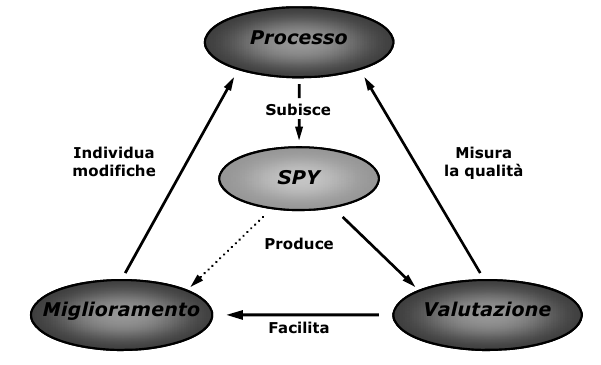
\includegraphics[width=.6\textwidth]{spy}
\caption{Il modello SPY per la valutazione della qualità di processo.}\label{fig:spy}
\end{figure}

La qualità di processo è parte fondamentale del processo per garantire la qualità del prodotto, e viene controllata ponendo come riferimento una serie di attributi specifici:

\begin{description}
\item \inglese{\textbf{Process performance}}: un processo raggiunge gli obiettivi prefissati trasformando input identificabili in output identificabili;

\item \inglese{\textbf{Performance managment}}: un processo è pianificato e controllato allo scopo di produrre risultati coerenti e corrispondenti agli obbiettivi per cui è stato attuato;

\item \inglese{\textbf{Work product management}}: un processo è pianificato e controllato allo scopo di produrre risultati documentabili, controllati e verificabili;

\item \inglese{\textbf{Process definition}}: l'attuazione di un processo si basa su un approccio stardardizzato;

\item \inglese{\textbf{Process resource}}: ogni processo ha a disposizione le adeguate risorse per essere attuato;

\item \inglese{\textbf{Process measurement}}: le misure e i risultati rilevati durante l'attuazione di un processo vengono usati per assicurarsi che lo stesso avvenga per raggiungere efficacemente gli obiettivi prefissati;

\item \inglese{\textbf{Process control}}: ogni processo è controllato mediante la raccolta, l'analisi e l'utilizzo delle misure di processo e di prodotto, al fine di valutare ed eventualmente correggere le sue modalità di attuazione;

\item \inglese{\textbf{Process change}}: il controllo sulle modifiche di gestione, attuazione o definizione di un processo è costante;

\item \inglese{\textbf{Continuous improvement}}: le modifiche e gli accorgimenti su un processo sono identificati e implementati allo scopo di assicurare il continuo miglioramento al fine di raggiungere più efficacemente gli obbiettivi rilevati.
\end{description}

Il modello fornisce inoltre una scala di valutazione sul grado di maturità dei processi, composta da cinque livelli e riportata in figura~\ref{fig:cmmi}. Il livello raggiunto dai fornitori viene utilizzato come ``biglietto da visita'' nella candidatura ai bandi. Questo significa che quanto più elevato è il livello raggiunto dal fornitore tanto migliore è la presentazione che offre di se stesso sullo specifico processo.

\begin{figure}[h]
\centering
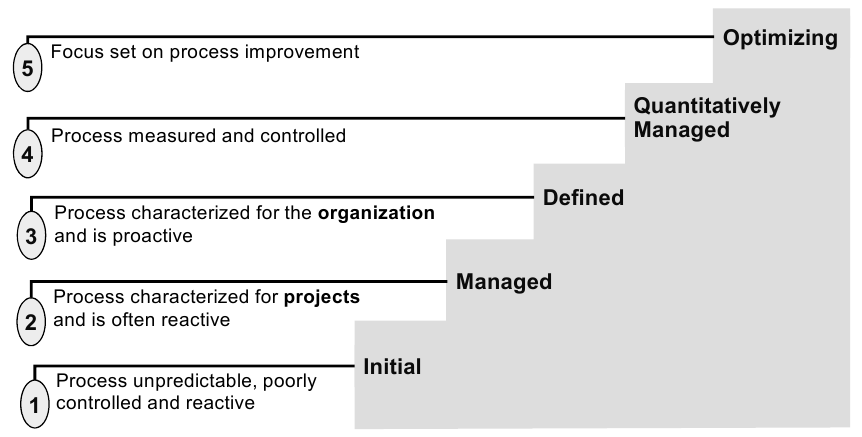
\includegraphics[width=.7\textwidth]{cmmi}
\caption{I livelli della classificazione CMMI.}\label{fig:cmmi}
\end{figure}

\begin{itemize}
\item \textbf{Livello 0}: processo non implementato o incapace di raggiungere gli obiettivi prefissati, non vi è inoltre evidenza di alcun approccio sistematico agli attributi definiti;

\item \textbf{Livello 1}: Il raggiungimento di questo livello è dimostrato attraverso l'attributo specifico \inglese{Process performance} in quanto il processo è messo in atto e raggiunge gli obbiettivi prefissati, tuttavia non è evidente nessun approccio sistematico per nessuno degli attributi definiti. 

\item \textbf{Livello 2}: ll raggiungimento di questo livello è dimostrato attraverso il possesso degli attributi di \inglese{Performance management} e \inglese{Work product management}. Il processo è gestito e sulla base di obbiettivi definiti è pertanto attuato, pianificato, tracciato, verificato ed eventualmente corretto.

\item \textbf{Livello 3}: ll raggiungimento di questo livello è dimostrato attraverso il possesso degli attributi di \inglese{process definition} e \inglese{process resource}. Il processo è definito e sulla base di procedure definite sui principi del \inglese{software engineering} è pertanto attuato, pianificato e controllato.

\item \textbf{Livello 4}: ll raggiungimento di questo livello è dimostrato attraverso il possesso degli attributi di \inglese{process measurement} e \inglese{process control}. Il processo risulta ora predicibile, è stabilizzato ed attuato e rispetta i risultati attesi nonchè le performance e le risorse impiegate.

\item\textbf{Livello 5}: ll raggiungimento di questo livello è dimostrato attraverso il possesso degli attributi di \inglese{process change} e \inglese{continuous improvement}. Il processo si presta all'ottimizzazione, è predicibile e in grado di adattarsi al raggiungimento di obbiettivi specifici e rilevanti a livello organizzativo.
\end{itemize}
\clearpage
%il clearpage serve solo a rendere più leggibile il testo, se modifichiamo il pezzo sopra verrà tolta.

La qualità dei processi, come già accennato ad inizio sezione, è una condizione necessaria per arrivare ad un prodotto di qualità. Il team si pone l'obiettivo di garantire e ottimizzare la qualità dei propri processi mediante l'utilizzo di strumenti necessari per garantirla, pertanto si aspetta di trarre da tali considerazioni:

\begin {itemize}
\item [-] un ottimizzazione dell'uso delle risorse;
\item [-] una migliore gestione economica, contenendo al massimo i costi;
\item [-] una maggiore possibilità di confronto con delle \inglese{best practice};
\item [-] maggiore affidabilità nei tempi di stima rispetto alle consegne preventivate;
\item [-] una migliore stima dei rischi e la loro gestione;
\end {itemize}

Inoltre ogni processo sarà definito in modo dettagliato e valutato l'output prodotto. Infine verranno attuate procedure di misurazione, valutazione ed eventuale modifica sul processo per perseguire il suo miglioramento mediante una costante collaborazione tra il verificatore e lo sviluppatore del processo stesso.

\subsection{Qualità di prodotto software}
Al fine di garantire un elevato standard qualitativo, sia per ovvia scelta del team di sviluppo, sia per implicita richiesta da parte del committente stesso, \team{} ha preso come riferimento lo standard ISO/9126:2001.

\begin{description}
\item{\bfseries Funzionalità}
Il prodotto \caName{} deve soddisfare nelle sue funzionalità tutti i requisiti obbligatori individuati nell'attività di analisi, garantendone il funzionamento e l'aderenza alle richieste specifiche del committente. Tutto questo sarà svolto nel modo meno oneroso sia dal punto di vista economico che di sfruttamento delle risorse disponibili.

Per valutare il grado di funzionalità raggiunto dal prodotto si valuterà la quantità di requisiti che sono stati correttamente implementati all'interno del software finale. La soglia minima di soddisfacimento risulta essere l'assoluta copertura dei requisiti obbligatori imposti dal committente, tuttavia è parso chiaro che la fantasia del team in questa specifica area sarà ben valutata.

\item{\bfseries Portabilità}
Il prodotto finale dovrà per vincoli di capitolato essere pianamente usufruibile mediante browser \underline{Chrome}, prodotto da Google, su tutti i sistemi operativi sui quali questo browser risulta compatibile.

A dimostrazione di tale soddisfacimento ci si affida alla dimostrazione del superamento della validazione del codice del \inglese{front-end web} e dell'assoluta coerenza con le specifiche \underline{WebRTC}, proposta evolutiva di \underline{HTML5}.
All'approvazione del superamento di tale requisito si procederà con lo stesso metodo testando browser alternativi a quello imposto al fine di rendere \caName{} usufruibile da un bacino d'utenza più vasto possibile.

\item{\bfseries Usabilità}
Il prodotto deve risultare facile ed intuitivo da parte dell'utenza che dispone di una conoscenza medio-bassa del web e dell'informatica in generale.

Utenti che hanno familiarità con programmi per la gestione di chiamate mediante \underline{VOIP} non dovranno trovare alcuna difficoltà o iniziale disorientamento nell'utilizzo di \caName{}.

Data l'aleatorietà di tale qualità di prodotto e la non ``oggettività'' nella misurazione di tale caratteristica si cercherà semplicemente di raggiungere tale risultato basandosi su esperienze personali o brevi test su specifici utenti selezionati.

\item{\bfseries Affidabilità}
L'applicazione deve riuscire a stabilire e mantenere stabile una comunicazione tra due o più utenti, senza mostrare problemi di natura tecnica se non imputabili alla qualità della connessione di cui dispongono gli utenti stessi. Deve dimostrarsi altresì robusta nella sua struttura e facile da ripristinare in caso di errori di varia natura.

Al fine di garantire queste caratteristiche verrà utilizzata come unità di misura la quantità di interazioni tra utenti con esito positivo, tenendo conto di tutti i parametri che concorrono ad una corretta comunicazione (qualità audio, video, messaggi testuali correttamente inviati/ricevuti, etc.).

\item{\bfseries Efficienza}
\caName{} si pone come obbiettivo oltre alla corretta ed appagante esperienza comunicativa, anche di non risultare particolarmente esosa dal punto di vista hardware, sia dal punto di vista puramente componentistico dell'unità dalla quale si accede al prodotto, sia dal punto di vista dell'uso di banda a disposizione della rete.

Verranno pertanto monitorate in fase di test sia le percentuali d'utilizzo di memoria e processore della macchina, sia la quantità di kb/s trasmessi e ricevuti durante l'esecuzione del programma. I test verranno eseguiti su varie tipologie di hardware e linee di diverse velocità, al fine di rendere il software usufruibile dalla più vasta fetta d'utenza possibile.

I test risulteranno superati se nei momenti di massimo consumo di risorse il programma riuscirà a garantire un utilizzo fluido e una discreta navigabilità nel web dalla macchina soggetta al test. 

\item{\bfseries Manutenibilità}
Il capitolato specifica esplicitamente che la modifica e la manutenibilità del software sono una caratteristica fondamentale dell'intero progetto, questa necessità nasce dal costante utilizzo di linguaggi non ancora qualificati come standard, pertanto soggetti a continua evoluzione.
\end{description}

\subsubsection{Ciclo di Deming}
Per riscontrare e raggiungere le caratteristiche sopra elencate il team ha deciso di adottare il \underline{ciclo di Deming} (PDCA)\@.

\begin{figure}[h]
\centering
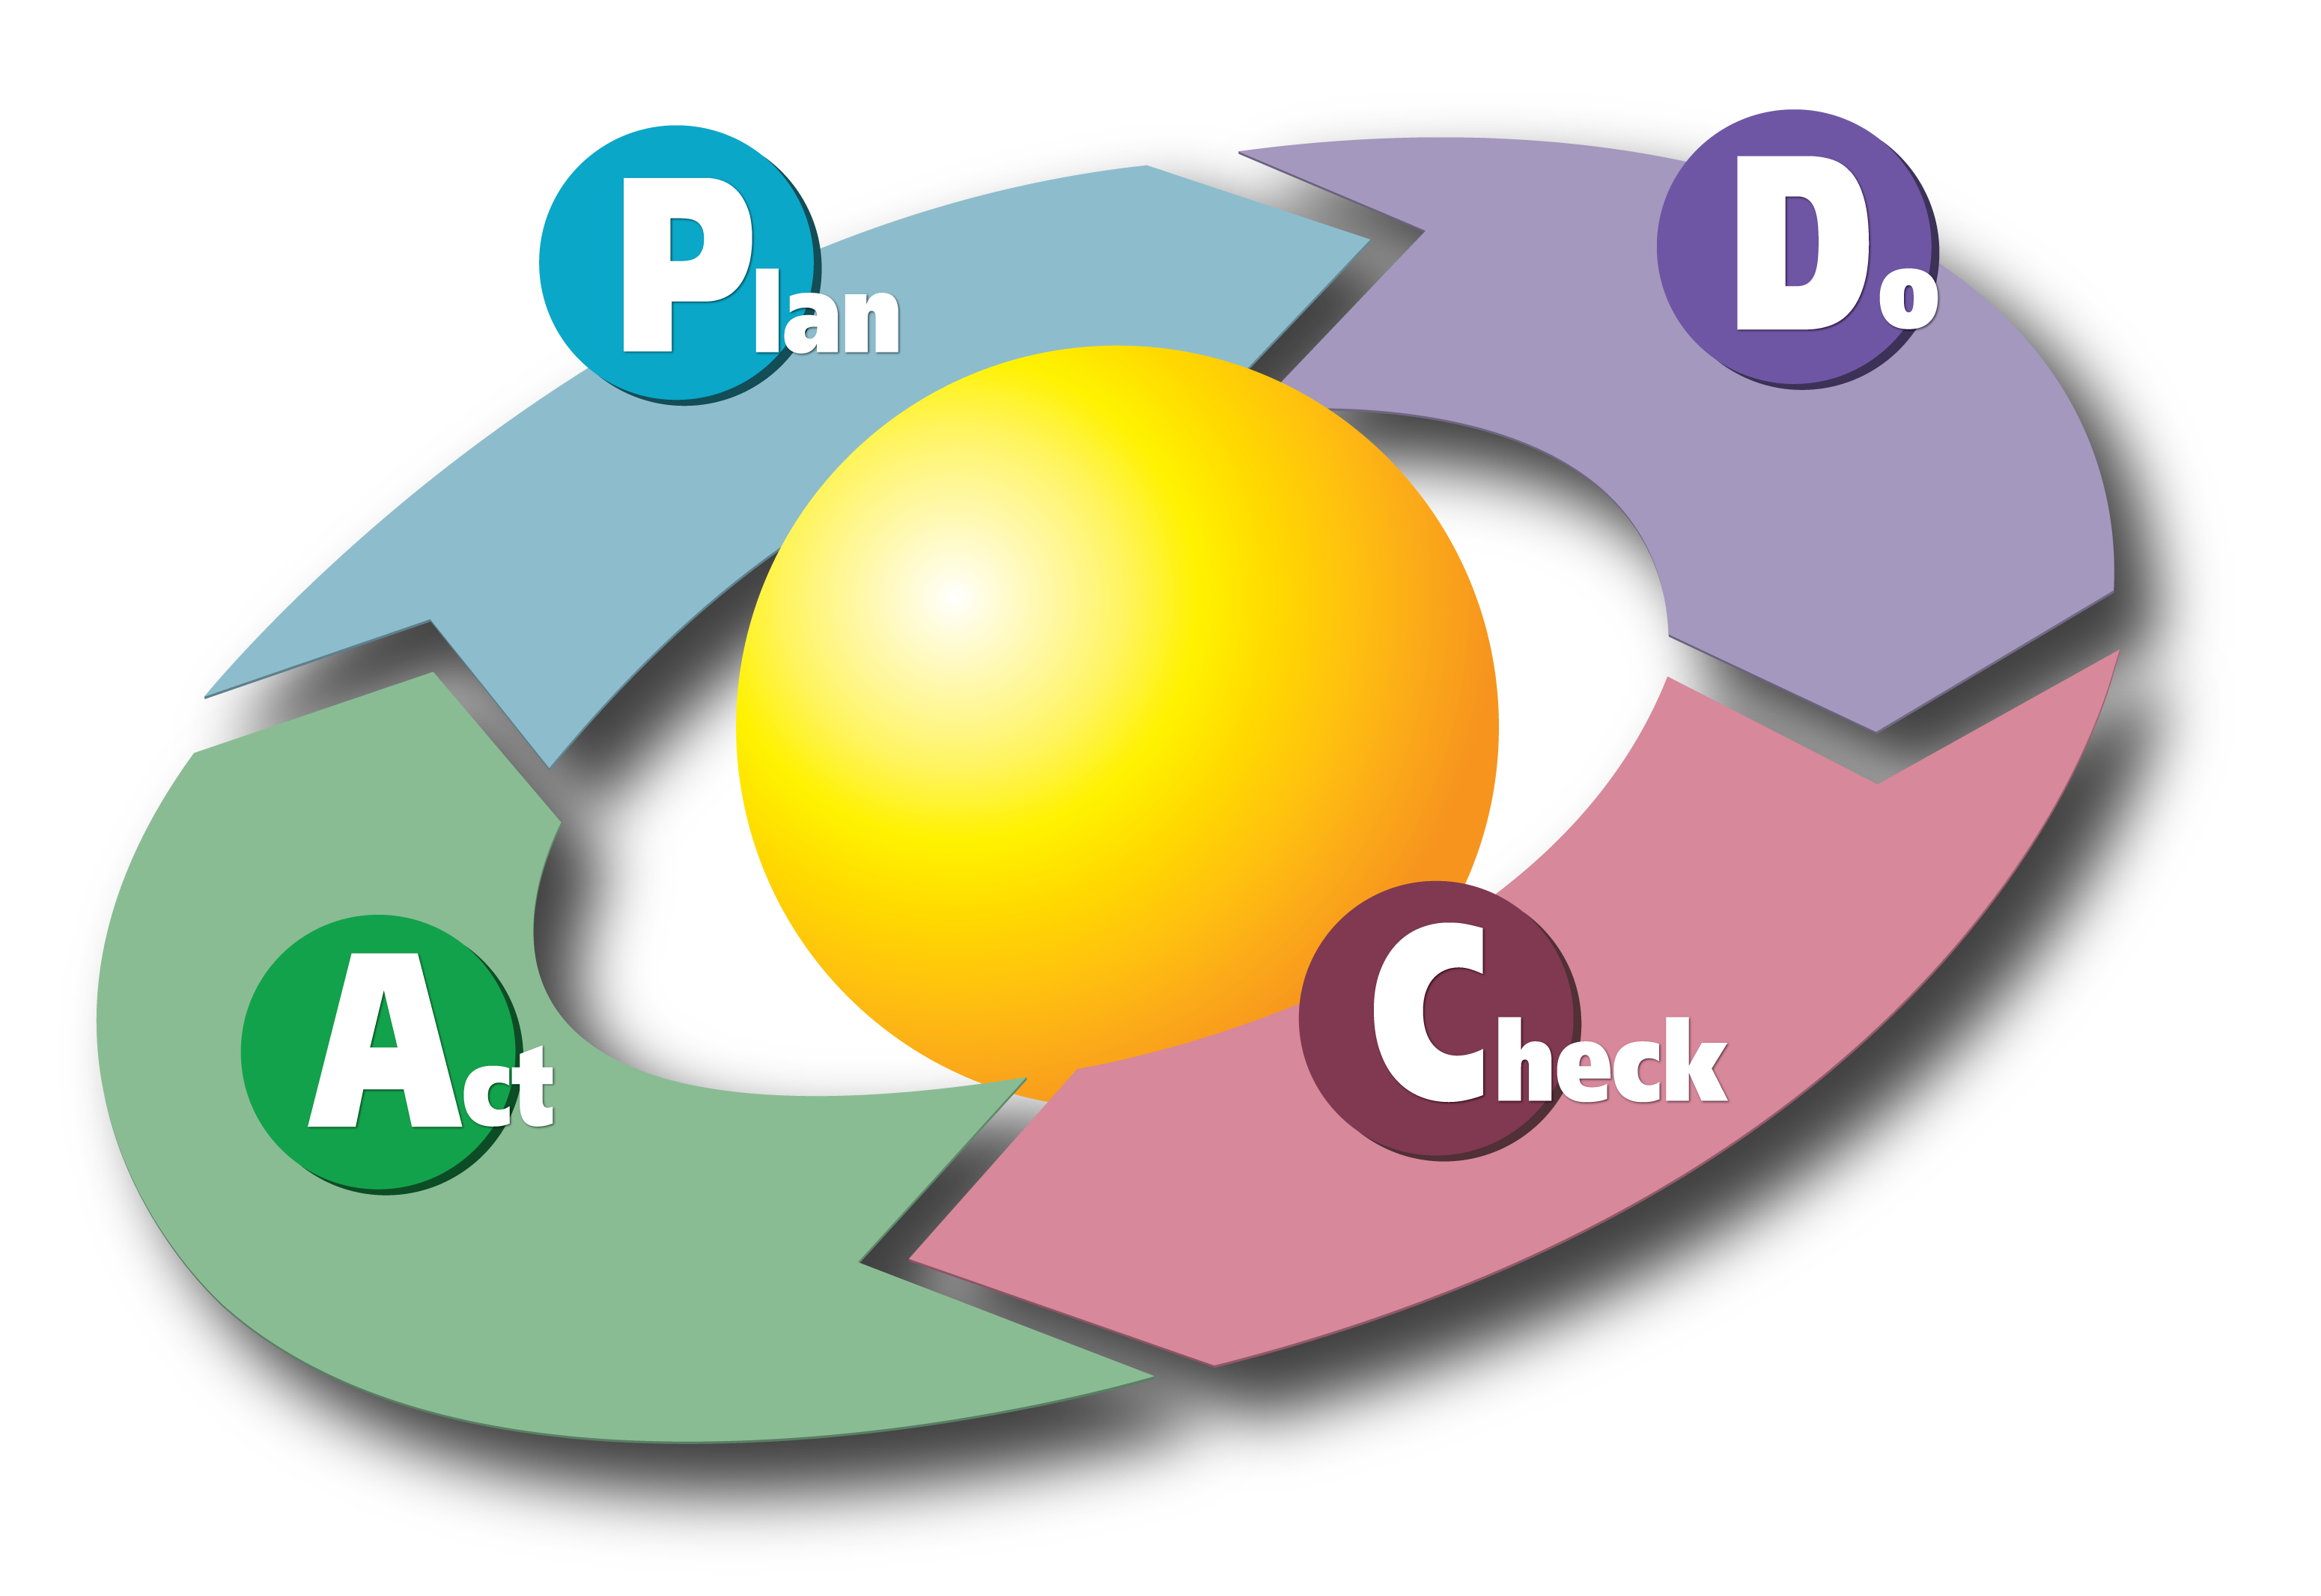
\includegraphics[width=.35\textwidth]{pdca}
\caption{Il ciclo di Deming.}\label{fig:pdca}
\end{figure}

Tale tecnica è costituita dalle seguenti fasi:

\begin{tabularx}{.9\textwidth}{>{\bfseries\scshape}lX}
plan  & analizzare il problema e stabilire le attività, le tempistiche e i soggetti coinvolti;\\
do    & attuare dettagliatamente le attività pianificate;\\
check & verificare a consuntivo quanto preventivato nella pianificazione;\\
act   & nel caso in cui il controllo abbia rilevato discrepanze tra preventivo e consuntivo attuare misure correttive.\\
\end{tabularx}

Gli obiettivi di qualità prefissati possono essere raggiunti tramite una adeguata pianificazione delle attività, che deve essere rispettata attentamente per poter permettere l'autovalutazione ed eventualmente l'adozione di misure correttive volte al miglioramento continuo e all'attuazione delle \underline{\inglese{best practices}}.  Solo in tal modo è infatti possibile ottenere un prodotto di qualità.

\subsection{Gestione della qualità}
La qualità di un software non si limita all'assenza di problematiche durante il suo funzionamento  anche se è evidente che la maggior parte delle attività inerenti al suo controllo hanno come fine ultimo l'identificazione e l'eliminazione di ogni possibile caratteristica che si discosti dal comportamento atteso del programma o dai requisiti che il programma stesso deve soddisfare.

Al fine di rendere ancor più chiara la comprensione di tali problematiche ed evitare che termini all'apparenza simili assumano significati impropri precisiamo che un \underline{\textbf{malfunzionamento}} è un funzionamento di un programma (o di una sua parte) diverso da quanto previsto dalla sua specifica, un \underline{\textbf{difetto}} è la causa di un malfunzionamento, mentre un \textbf{errore} è l'origine di un difetto.
Tali termini oltre ad avere un significato diverso hanno quindi anche una dipendenza causa-effetto gli uni dagli altri, con una dipendenza temporale ben definita.

Terminiamo il capitolo evidenziando gli aspetti fondamentali per contenere i problemi descritti in precedenza e accertare la qualità del prodotto e dei processi: \inglese{Quality Assurance}, Verifica e validazione.
Nel primo caso si intende l'insieme della attività svolte a garantire il soddisfacimento degli obbiettivi di qualità prefissati, mentre la verifica deve garantire che avvengano i controlli affinché il prodotto ottenuto al termine di una fase sia coerente con quanto precedente a tale fase. La Validazione è infine un'attività di controllo che confronta il risultato di una fase del processo di sviluppo del prodotto con i requisiti del prodotto stesso.\\

Verifica e validazione sono attività che coesistono con quelle tradizionali, e la loro integrazione deve essere svolta nel modo più efficace possibile al fine di renderle concretamente produttive in quanto la scoperta di un errore durante lo sviluppo garantisce un guadagno significativo per la qualità del prodotto.
\clearpage

\section{Visione generale della strategia di verifica}

\subsection{Organizzazione, pianificazione strategica, pianificazione temporale e responsabilità}
L'attività di verifica inizierà quando il prodotto di un processo raggiungerà uno stadio che si potrà definire diverso da quello precedente a seguito della conclusione di un processo di ciclo di vita.

La verifica di tali cambiamenti sarà operata in modo mirato e circoscritta, grazie al registro delle modifiche che verrà compilato durante la stesura del documento stesso. Al termine della fase di verifica, i documenti saranno consegnati al responsabile di progetto, che provvederà ad approvarli.

Il team nel \underline{\inglese{brainstorming}} successivo all'analisi generale del progetto \caName{} ha deciso di adottare un ciclo di vita incrementale (specificato nel documento \textit{piano\_di\_progetto.3.0.pdf}).

Coerentemente a tale scelta, il processo di verifica adottato opererà nelle diverse fasi del progetto nel modo seguente:

\subsubsection{Analisi dei Requisiti}
Quando un documento uscirà dalla fase di redazione, verrà preso in esame ed effettuata una fase di revisione definitiva prima di essere presentato ufficialmente alla RR: 
\begin{itemize}
  \item[-] Verrà presa in esame la correttezza grammaticale, che al contrario di quella ortografica può essere verificata solo mediante un accurata rilettura da parte del verificatore designato.
  \item[-] Verrà presa in esame la correttezza lessicale mediante un'accurata rilettura da parte del verificatore designato.
  \item[-] Verrà presa in esame la correttezza dei contenuti e la coerenza rispetto al documento mediante un accurata rilettura da parte del verificatore designato.
  \item[-] Verrà effettuata la verifica che ogni tabella o figura sia corretta nel suo contenuto e disponga della rispettiva didascalia.
  \item[-] Verrà presa in esame la correttezza rispetto alle norme di progetto redatte, utilizzando gli strumenti più appropriati per la verifica.
  \item[-] Verrà presa in esame la corrispondenza tra ogni requisito e i casi d'uso, consultando e controllando le apposite tabelle di tracciamento, verificando inoltre la corretta gestione di entrambi mediante \manager, l'applicativo web creato appositamente da \team.
  \item[-] Verrà considerata la corrispondenza fra i requisiti elencati e quanto enunciato nel testo del capitolato, in modo da assicurare che tutti i requisiti espliciti siano stati correttamente recepiti.
  \item[-] Verrà presa in esame la chiarezza espositiva nell'enunciazione dei requisiti al fine di ridurre al minimo le ambiguità nonché la granularità dei requisiti individuati, perché avere requisiti atomici ne rende più facile il tracciamento e la verifica del soddisfacimento.
\end{itemize}

\subsubsection{Progettazione}

\subsubsection*{Progettazione ad alto livello}
Il processo di verifica garantirà la rintracciabilità nei componenti individuati durante la fase di Progettazione architetturale di ogni singolo requisito descritto nel documento di analisi dei requisiti (versione 3.0). A tale scopo lo strumento che si è scelto di utilizzare è ancora \manager, nello specifico tramite il modulo relativo ai \inglese{configuration item}.

Tali verifiche verranno svolte al termine della stesura del documento di specifica tecnica e dell'aggiornamento dei documenti relativi al piano di progetto, piano di qualifica, norme di progetto, analisi dei requisiti.

Al fine di garantire un'elevata qualità nell'architettura software elaborata durante la progettazione di alto livello, la verifica dovrà valutare la presenza delle seguenti proprietà:
\begin{itemize}
\item \textbf{necessità} ogni componente soddisfa almeno uno fra i requisiti emersi in fase di analisi;
\item \textbf{sufficienza} l'architettura nel suo complesso è in grado di soddisfare tutti i requisiti;
\item \textbf{modularità} è chiaramente definita la suddivisione delle varie componenti e il ruolo di ciascuna di esse;
\item \textbf{flessibilità} permette modifiche a basso costo al variare dei requisiti;
\item \textbf{affidabilità} consente un utilizzo corretto durante il funzionamento;
\item \textbf{semplicità} ogni parte contiene tutto e solo ciò che è necessario al proprio funzionamento;
\item \textbf{incapsulamento} le parti del sistema mantengono private le informazioni relative al proprio stato interno e permettono di accedervi solo attraverso le operazioni dell'interfaccia pubblica che espongono verso l'esterno;
\item \textbf{coesione} le componenti che stanno assieme condividono lo stesso obiettivo;
\item \textbf{basso accoppiamento} eventuali modifiche a una componente avranno bassa o nulla incidenza sul resto dell'architettura grazie al controllo delle relazioni di dipendenza.
\end{itemize}

Infine, i diagrammi UML riportati nel documento di specifica tecnica saranno sottoposti a verifica rispetto a quanto stabilito nella sezione 3.4 del documento \textit{norme\_di\_progetto.3.0.pdf}.

\subsubsection*{Progettazione di dettaglio}
Per ogni unità architetturale prodotta durante la fase di progettazione di dettaglio verrà effettuato un test di unità al fine di verificarne il comportamento dell'unità stessa rispetto a quello atteso in fase d'esecuzione. Tali test sono definiti da:
\begin{itemize}
  \item un oggetto su cui viene eseguito e gli obbiettivi del il test;
  \item la strategia e le risorse software utilizzate nella prova;
  \item il piano d'esecuzione del test stesso.
\end{itemize}

Allo scopo di ridurre al minimo la presenza di errori interni alle singole unità sono stati programmati un numero di test sufficiente ad assicurare \inglese{statement coverage} e \inglese{branch coverage}, la prima ha lo scopo di assicurare che tutte le linee di comando di ciascun modulo siano state eseguite almeno una volta, mentre la seconda assicura che tutti i possibili rami del flusso di controllo vengono attraversati almeno una volta.

Effettuati i test di unità si procederà con l'unione delle unità stesse in modo da poter effettuare i relativi test d'integrazione per verificare come le varie componenti del sistema interagiscono tra loro, evidenziando eventuali difetti di progettazione, e dipendenze (o incompatibilità) tra i diversi componenti architetturali.

La pianificazione dei vari test da eseguire verrà fornita dal team \team{} una volta terminata la fase di progettazione di dettaglio.

\subsubsection{Codifica}
I programmatori svolgeranno le attività di codifica del prodotto e i test di unità per la verifica del codice realizzato nel modo più automatizzato possibile.

I verificatori inoltre controlleranno la presenza di eventuali discrepanze rispetto alle norme pattuite in merito al processo di codifica, nonché l'identificazione di parti di codice soggette ad errori di programmazione.
I modelli presi in considerazione per eseguire tali verifiche sono due: verifica funzionale e verifica  strutturale.

La verifica funzionale (\underline{\inglese{black-box}}) è una tecnica che procederà con l'accertamento delle funzionalità di un unità controllando esclusivamente che i risultati in uscita rispecchino il valore atteso in ogni condizione d'utilizzo che l'unità dispone. Questo tipo di modello consente test efficaci sull'intero sistema o su unità di dimensioni rilevanti.

La verifica strutturale (\underline{\inglese{white-box}}) al contrario è una tecnica in cui l'ispezione viene svolta a livello di codice sorgente, richiamando esplicitamente tutti i metodi presenti nell'unità al fine di verificarne, oltre al corretto funzionamento, anche la correttezza logica. Questo modello si predilige per controlli sui singoli moduli che costituiscono il progetto, controllando come già citato la struttura stessa del codice.

Specifichiamo infine che per effettuare un controllo approfondito del codice si utilizza il termine ``analisi'', che si specializza essenzialmente in due tipologie: analisi statica e dinamica.

L'analisi statica non comporta l'esecuzione del codice in quanto la verifica avviene tramite lettura da parte di un verificatore (tramite \underline{\inglese{inspection}} e \underline{\inglese{walkthrough}}, descritti più dettagliatamente nella sezione 5.1.1) o mediante opportuni strumenti software di verifica statica. Gli errori riscontrati mediante tali metodologie dal verificatore non vengono corretti dal soggetto stesso, ma vengono riferiti al progettista o al programmatore al quale comunque rimane il compito di individuazione e correzione degli errori individuati durante il suo lavoro sul codice stesso.
L'analisi dinamica richiede l'esecuzione del programma in un ambiente controllato e con dati in ingresso verificati. Verranno registrati tutti i dati relativi all'esecuzione e inerenti alla quantificazione della qualità del software preso in esame, inoltre tali dati saranno confrontati con i requisiti stilati.

    
\subsubsection{Validazione}
Alla fase di collaudo, il team garantirà il corretto funzionamento del prodotto \caName{} relativo alle funzionalità,l'usabilità, l'efficienza, l'affidabilità, e la portabilità. Tali garanzie vengono confermate dopo un'attività interna di test denominata Alfa-test. All'esito positivo di tale attività avverrà il collaudo vero e proprio (Beta-test) alla presenza del proponente, successivi \underline{difetti} riscontrati o eventuali caratteristiche non coerenti alle richieste di quest'ultimo saranno soggette a modifica e correzione al fine di eliminare tali incongruenze.
\clearpage

\subsection{Risorse necessarie e disponibili}
L'utilizzo di risorse umane e tecnologiche è fondamentale per la verifica di qualità del prodotto e dei processi.

\subsubsection{Umane}
\team{} si è imposta, per garantire un elevato standard qualitativo, che all'interno del team siano ricoperti, nel corso del progetto, i seguenti ruoli:

\begin{itemize}
\item Responsabile: responsabile della corretta realizzazione del prodotto secondo gli standard e le richieste commissionate, designato all'allocazione corretta delle risorse umane ai rispettivi compiti e stimolarne il coordinamento. 
Controlla inoltre la qualità dei processi interni mediante le attività di verifica da lui predisposte. Infine ha la facoltà di approvare o meno ogni proposta di correzione (migliorativa o di modifica generica) avanzata.
\item Amministratore: stila le metodologie e definisce le norme per la verifica dei processi, gestisce inoltre i risultati relativi ai test eseguiti e il processo di gestione e correzione delle anomalie e delle discrepanze.
\item Verificatore: applica i processi di verifica e validazione approvati dall'amministratore e predisposte dal responsabile tenendo traccia del suo lavoro. Ogni discrepanza o anomalia incontrerà durante tale attività verrà presentata tramite \inglese{ticketing} (vedi capitolo 5 del documento \textit{norme\_di\_progetto.3.0.pdf}).
\item Programmatore: durante il suo lavoro ha l'obbligo di risolvere le anomalie evidenziate tramite \inglese{ticketing} dai verificatori o dai test effettuati sul codice da lui stesso prodotto.
\end{itemize}

\subsubsection{Software}
A livello software risulteranno necessarie, le seguenti risorse:

\begin{description}
\item{\bfseries \manager}, il programma basato su interfaccia web sviluppato internamente al team per il tracciamento e la gestione dei requisiti avente lo scopo di standardizzare e rendere quanto più automatizzata possibile tale fase del progetto ed evitare quindi l'insorgere di eventuali sviste dovute all'intervento umano.

\item{\bfseries Sistema di controllo versione} (in particolare \texttt{git}) al fine di permettere il lavoro in parallelo da parte dei membri del gruppo e la gestione dello storico delle versioni; il gruppo prevede altresì di appoggiarsi a un \underline{\inglese{repository}} remoto per permettere la sincronizzazione fra i diversi utenti (cfr.~sez.~3.1 del documento \textit{norme\_di\_progetto.3.0.pdf}). 

\item{\bfseries Editor di diagrammi}, da impiegarsi tanto per la produzione dei diagrammi UML richiesti per l'attività di progettazione quanto per la creazione dei diagrammi di Gantt necessari alla pianificazione delle attività di progetto. 

\item{\bfseries \underline{Sistema di \inglese{ticketing}}}, per gestire la suddivisione e l'assegnazione delle attività ai vari componenti del gruppo in maniera ordinata e controllabile.

\item{\bfseries Ambiente di sviluppo integrato (\underline{IDE})}, al fine di individuare e correggere già durante l'attività di codifica gli eventuali errori presenti nel codice nonché di renderne più agevole la ristrutturazione (\inglese{refactoring}).

\item{\bfseries Analizzatori statici}, vale a dire strumenti per permettere l'automatizzazione nell'analisi del codice prodotto, ai fini di ricavarne il maggior numero possibile di informazioni. Le risorse da utilizzare a tale scopo sono descritte con maggiori dettagli nella sezione~8.1 delle norme di progetto (versione 2.0).

\item{\bfseries \inglese{Testing framework}}, che risulteranno utili ai fini dei test di unità legati al linguaggio di programmazione scelto per standardizzare (e automatizzare) i test sul prodotto finale nonché produrre dei resoconti appropriati sulle eventuali anomalie riscontrate.

\item{\bfseries \inglese{Editor} di documenti}, secondo quanto documentato nella sezione~4.1 delle norme di progetto (versione 2.0), in particolare un editor di testo specializzato per \LaTeX con evidenziazione della sintassi, autocompletamento dei comandi e correzione ortografica integrata. 
\end{description}

Gli specifici programmi e \inglese{tool} per la gestione di tali servizi sono descritti in dettaglio nel documento \textit{norme\_di\_progetto.3.0.pdf} allegato.

\subsubsection{Hardware}
\team{} ha a disposizione oltre al materiale personale di ogni componente del team (computer portatili e fissi) le strutture fisiche ed informatiche messe a disposizione dalla facoltà di informatica dell'Università degli Studi di Padova, quali laboratori didattici e le aule studio allocate negli stabili della Facoltà stessa.
\clearpage


\section{Tecniche, metodi e metriche}

\subsection{Tecniche}
Durante lo svolgimento del progetto il team utilizzerà le tecniche di analisi statica e dinamica per effettuare verifiche su software e documentazione.

\subsubsection{Analisi statica} 
L’analisi statica è un tipo di controllo basato sulla non esecuzione del codice, ma in senso lato può essere applicato a qualsiasi tipo di prodotto anche non propriamente eseguibile (ad es. la documentazione di progetto). Sono previste, in particolare, due forme di analisi statica: il controllo manuale (detto altrimenti \inglese{desk check}) e il controllo assistito da strumenti automatici.
Per quanto concerne il \inglese{desk check}, cioè il controllo realizzato unicamente da parte di un agente umano, sono previsti due metodi formali:

\begin{itemize}
\item \textbf{\underline{walkthrough}}: implica un esame ad ampio spettro del prodotto da verificare, che è preso in considerazione nella sua totalità in modo indiscriminato e senza alcuna assunzione previa sulla natura, la posizione e la frequenza degli errori da rilevare. Si tratta notoriamente di una tecnica molto onerosa in termini sia di tempo che di sforzo e può essere essa stessa per sua natura soggetta ad errori (in particolar modo falsi negativi). Tuttavia, almeno nelle fasi iniziali del lavoro, è l’unica scelta praticabile a causa della relativa inesperienza dei membri del gruppo nella realizzazione di prodotti complessi e articolati (sia software che documentazione). Allo scopo di ridurre il costo determinato dalla ripetizione di tale attività nell'arco di tutto il ciclo di vita è previsto che durante l’analisi in \inglese{walkthrough} sia stilata una lista di controllo relativa agli errori più frequenti e ai contesti in cui è più probabile che si producano errori in modo da collezionare una base di esperienza comune e consolidata destinata ad alimentare le attività di ispezione.

\item \textbf{\underline{inspection}}: prevede un controllo mirato avente obiettivi specifici, ristretti e stabiliti a priori \textit{prima} che la verifica abbia luogo. Si tratta di un’attività meno dispendiosa in termini di risorse perché non presuppone l’analisi esaustiva del prodotto ma è focalizzata su determinate categorie di errori frequenti, enunciate in una lista di controllo (\inglese{checklist}) redatta sulla base dell'esperienza personale e delle attività di \inglese{walkthrough} precedentemente poste in essere.
\end{itemize}


\subsubsection{Analisi dinamica} 
I controlli dinamici, altrimenti definiti test, prevedono l’esecuzione del software in un ambiente controllato e con dati di input specificatamente pensati per testarne le funzionalità e l’aderenza ai requisiti mettendo in luce l’eventuale presenza di malfunzionamenti dovuti alla presenza di difetti.

Caratteristica fondamentale dei test è la loro \textbf{ripetibilità}, cioè dato lo stesso set di dati in ingresso e nello stesso contesto di esecuzione, l’output deve essere deterministico e univocamente determinato. Tale proprietà, unitamente all'auspicabile utilizzo di un \inglese{logger} che ha il compito di registrare le fasi dell'esecuzione del test, consente di individuare e riconoscere in maniera più agevole i difetti presenti nel prodotto.

In base al loro ambito di applicazione, i test possono essere suddivisi in:
\begin {itemize}
\item test di unità aventi come oggetto le singole unità e, oltre al modulo da verificare e ai dati d’esempio, possono coinvolgere anche componenti attive (\underline{driver}) o passive (\underline{stub}) che siano in grado di simulare le parti del sistema non ancora disponibili al momento in cui il test viene eseguito;

\item test di integrazione atti a verificare la corretta interazione e integrazione fra le componenti che costituiscono le parti del sistema e hanno come risultato una \inglese{build}, vale a dire un sottosistema funzionante che può essere eseguito in modo indipendente;

\item test di sistema, volti a testare il rispetto dei requisiti software individuati in fase di analisi dei requisiti da parte dell’intero sistema;

\item test di regressione destinati a rilevare il caso indesiderabile in cui una modifica locale destabilizza il resto del sistema, si tratta del numero minimo di test necessario per scongiurare tale eventualità senza per questo dover ripetere in toto i test di unità e di integrazione;

\item test di accettazione, o collaudo, realizzato sotto la supervisione del committente per verificare l’aderenza del prodotto ai requisiti utente di più alto livello.

\end{itemize}

\subsection{Metodi}
Il processo di misurazione attraverso il quale è possibile valutare quantitativamente l'aderenza del prodotto agli standard di qualità è basato su un ciclo iterativo simile al ciclo di Deming. In particolare, in una fase preliminare prevede che sia stabilita l'importanza e l'ambito di applicazione della misurazione, la selezione di metriche da adottare come si è fatto nelle precedenti sezioni e la pianificazione del momento nel ciclo di sviluppo in cui le misurazioni dovranno essere effettuate.

La parte operativa, cioè la quantificazione dei valori delle metriche di qualità, avviene lungo tutto l'arco del ciclo di sviluppo, con particolare attenzione alle fasi di progettazione di dettaglio e di test effettuati contestualmente alla codifica e in fase di accettazione/collaudo.

Al fine di evitare che la verifica della qualità sia un onere troppo gravoso in termini di risorse umane e di tempo, anch'esso deve essere sottoposto a misurazione in quanto attività di progetto (cioè la parte \inglese{check} di PDCA): il tempo di lavorazione impiegato per attività di verifica e \underline{QA} dovrà dunque essere registrato in ogni momento, ed è prerogativa del responsabile di progetto adottare misure correttive qualora i tempi dovessero risultare eccessivi al punto da compromettere il rispetto delle scadenze stabilite nel piano di progetto.

Il team ha quindi, dopo aver analizzato il problema che andrà ad affrontare, optato per utilizzare le seguenti tipologie di analisi statica: 
\begin{itemize}

\item \textbf{Analisi di flusso di controllo:} il prodotto sviluppato avrà caratteristiche di affidabilità e robustezza, riducendo al minimo gli sprechi. Questa analisi ha il compito di verificare che il codice sia eseguito nella giusta sequenza, correttamente strutturato, e non siano presenti parti di codice non raggiungibili o iterazioni aventi un limite superiore non definito. A tale fine sarà necessario prestare particolare attenzione alle decisioni interne all'unità di codice e verificare che le condizioni risultino totalmente gestite.

\item \textbf{Analisi di flusso dei dati:} al fine di garantire che in ogni stato in cui si trova il prodotto si riesca ad accedere correttamente ai dati richiesti dall'utente e che nessun cammino d'esecuzione acceda a variabili prive di valore. 
Questa tipologia di analisi può rilevare anomalie quali scritture successive su una variabile senza letture intermedie o la presenza di variabili \inglese{write-only}. Al fine di evitare complicazioni inutili, per questo tipo di analisi si opterà per sconsigliare l'uso di variabili globali in fase di progettazione e codifica.

\item \textbf{Analisi di flusso di informazione:} per controllare il grado di accoppiamento, determinando le dipendenze tra ingressi e uscite che risultano dall'esecuzione di un'unità di codice e consentendo solo quelle previste dalla specifica degli specifici moduli.

\item \textbf{Verifica formale del codice:} garantisce la correttezza del codice sorgente sviluppato rispetto alla specifica formale dei requisiti redatta nell'attività di analisi.
\end{itemize}

\subsection{Metriche}
Per effettuare delle misure efficacemente è necessario definire un'unità di misura, una scala metrica e il metodo per rilevare tali misure.

Tali caratteristiche sono definite dettagliatamente dallo standard ISO/IEC 9126, e le metriche descritte possono essere catalogate secondo due macro categorie: metriche elementari e derivate. Le prime sono in grado di rappresentare istantaneamente un dato fenomeno, le metriche derivate al contrario sono ricavate da operazioni su altre misurazioni.

Sempre in riferimento alla capacità di immediatezza di misurazione sulle caratteristiche del prodotto si possono distinguere metriche dirette, che sono rilevabili sul software senza considerare l'influenza di fattori esterni (come l'ambiente nel quale è eseguito il software), e metriche indirette che combinano nelle misurazioni sul prodotto anche misure relative a elementi ambientali.

\subsubsection{Metriche per il progetto}
Relativamente all'andamento e alla gestione del progetto il team ha stabilito di affidarsi a una serie di indicatori al fine di ottenere una stima delle caratteristiche che per loro natura non possono essere misurate in maniera esatta. L'uso di tali indicatori è stato ritenuto opportuno al fine di valutare l'insorgenza di fattori di criticità e controllare il rispetto dei vincoli in termini di risorse (tempi/costi) di progetto.

Gli indicatori selezionati come candidati per l'utilizzo sono, in particolare:
\begin{description}
  \item{\scshape\bfseries BCWS} (\inglese{Budgeted Cost of Work Scheduled}) pari al costo preventivato in termini di ore per realizzare i \inglese{task} di progetto fino alla data corrente;
  \item{\scshape\bfseries ACWP} (\inglese{Actual Cost of Work Performed}) dato dal costo a consuntivo in termini di ore effettivamente impiegato per lo svolgimento dei \inglese{task} di progetto alla data corrente;
  \item{\scshape\bfseries BCWP} (\inglese{Budgeted Cost of Work Performed}) determinato dal valore delle attività terminate alla data corrente;
  \item{\scshape\bfseries BV} (\inglese{Budget Variance}) definito come \[BV \stackrel{\Delta}{=} BCWS - ACWP \] ovvero lo scostamento fra quanto preventivato e quanto sostenuto in termini di costi alla data corrente;
  \item{\scshape\bfseries CV} (\inglese{Cost Variance}) definito come \[BV \stackrel{\Delta}{=} BCWP - ACWP \] dato dallo scostamento fra il valore di quanto effettivamente prodotto dalle attività di progetto e il costo sostenuto.
\end{description}

\subsubsection{Metriche per la verifica del codice}\label{sec:metrics}

Si riporta un elenco delle principali metriche, in riferimento alle quali il team di sviluppo si ripropone di valutare in modo univoco e quantificabile la qualità del prodotto relativamente alla parte di codifica:

\begin{itemize}
  \item numero di righe di codice esclusi commenti e annotazioni, considerato nella sua totalità (TLOC, \inglese{Total lines of code}) o piuttosto come corpo dei soli metodi (MLOC, \inglese{Method lines of code});
  \item numero di metodi (NOM, \inglese{Number of Methods}) e numero di campi dati di ciascuna classe (NOF, \inglese{Number of Fields});
  \item profondità di una classe nell'albero di derivazione (DIT, \inglese{Depth of Inheritance Tree});
  \item numero di metodi ridefiniti (NORM, \inglese{Number of OverRidden Methods})
  \item indice di specializzazione (IS), definito come \[
  IS \stackrel{\Delta}{=} \frac{DIT \times NORM}{NOM}
  \]
  \item complessità ciclomatica, basata sul concetto che un metodo può essere rappresentato come un grafo, per calcolare tale complessità vengono sommati tutti i cammini linearmente indipendenti di tale metodo: maggiore è il numero di cammini, maggiore sarà di conseguenza la complessità ciclomatica e la possibilità che in tale codice ci siano errori; tale metrica è definita come
  \[v(G)=E-N+P\]
dove $E$ è il numero di archi, $N$ il numero di nodi e $P$ le componenti connesse da ogni arco e risulta essere molto utile per determinare il numero di test da effettuare su un determinato metodo per coprire tutti i cammini possibili;

  \item peso della classe (WMC, \inglese{Weighted Methods per Class}) definito come la somma della complessità ciclomatica di tutti i metodi membri di una classe;
  \item mancanza di coesione dei metodi di una classe (LCOM, \inglese{Lack of Cohesion of Methods}), un indice che misura quanto i metodi di una classe fanno riferimento ai campi dati della stessa, definito se $m(A)$ è il numero di metodi che riferiscono il campo dati $A$ come \[
  LCOM \stackrel{\Delta}{=} \frac{\frac{1}{NOF}\left(\displaystyle\sum_{A\;\mathrm{attributo}}{m(A)}\right) - NOM}{1-NOM}
  \]
  \item indice di utilità (Ca, \inglese{Afferent Coupling}) definito come il numero di classi esterne al package che dipendono da una determinata classe;
  \item indice di dipendenza (Ce, \inglese{Efferent Coupling}), definito come il numero delle classi interne al package che dipendono da una classe;
  \item instabilità (I) definita come \[
  I \stackrel{\Delta}{=} \frac{Ce}{Ca + Ce}
  \]
  \item astrattezza (a livello di progetto) dato dal rapporto fra il numero di classi astratte/interfacce e il numero totale di tipi;
  \item la metrica relativa a metodi e procedure $SFIN - SFOUT$, dove SFIN (\inglese{structural fan-in}) è il numero di volte che tale metodo è invocato nel corpo di altri metodi e SFOUT (\inglese{structural fan-out}) è il numero di invocazioni di metodi esterni all'interno del metodo stesso (corrispondono a Ca e Ce rispettivamente);
  \item rapporto fra righe di commenti e righe di codice.
\end{itemize}

Altre metriche che saranno prese in considerazione sono la lunghezza dei metodi e il numero di parametri di ciascun metodo.

\subsection{Misure}
Il processo di misurazione del software è normato dallo standard ISO di riferimento: ISO 15939 \inglese{Software Engineering - Software measurement process} (2002).

Tale processo è descritto come ciclo iterativo che prevede un'attività di misurazione, la raccolta di \inglese{feedback} derivata dai risultati e un'eventuale impostazione di azioni correttive per migliorare il processo produttivo.

Nel ciclo di vita del software, è possibile misurare lo stato raggiunto dal prodotto nei suoi vari stadi di lavorazione al fine di giungere a due previsioni distinte:
\begin{itemize}
 \item prevedere le caratteristiche del software in una fase del ciclo di vita diversa da quella in cui si sta effettuando la valutazione;
\item stimare le caratteristiche del software prodotto nello stadio di sviluppo raggiunto in cui si sta effettuando la valutazione.
\end{itemize}

Vi sono diversi momenti, durante tutti il ciclo di vita del progetto, che richiedono una valutazione delle caratteristiche del software che si sta producendo:
\begin{itemize}
\item \textbf{Fase di progettazione:} prevedere eventuali problemi nel software in un periodo temporale successivo al suo rilascio e quanto sarà facile eseguire eventuali interventi di manutenzione, valutandone l'impatto che avranno nel contesto d'utilizzo.

\item \textbf{Fase di collaudo:} confrontare che quanto prodotto sia coerente con le specifiche del committente, analizzando eventuali problemi che possono emergere e non sono stati considerati nell'attività di progettazione.

\item \textbf{Periodo successivo alla data di rilascio:} misurare l'impatto del software sull'efficienza e l'efficacia del lavoro svolto dall'utente che ne usufruisce, eventualmente confrontando il prodotto con eventuali concorrenti simili e valutandone potenziali aree di miglioramento, pianificando aggiornamenti mirati e creando, eventualmente, una versione migliorata del prodotto stesso.
\end{itemize}

Indispensabili sono inoltre delle misurazioni effettuate sia su entità semilavorate che compongono il prodotto software che sugli stati finali delle stesse. Si possono dividere tali misure in interne, che hanno una stretta dipendenza con le attività di sviluppo del prodotto, ed esterne, che non dipendono dalle fasi del ciclo di vita.

Le misure interne che si possono adottare sono:
\begin{itemize}

\item \textbf{Nell'analisi dei requisiti:} utili per stimare il costo del software e le implicazioni sul ciclo di vita del software, in questa fase si può misurare il numero di requisiti e di casi d'uso evidenziati.

\item \textbf{Nella progettazione:} stimano in modo più accurato il costo del software e alcuni aspetti inerenti alla qualità. In questa fase è possibile quantificare il numero di moduli in uno schema di progettazione e il loro livello di coesione ed accoppiamento.

\item \textbf{Nel codice:} come per le misure nella fase di progettazione si hanno stime a livello economico e qualitativo, misurando il numero di linee di codice prodotto, la complessità ciclomatica dello stesso, di coesione funzionale ed eventuali misure \inglese{object oriented} che valutano l'ereditarietà, il polimorfismo, l'incapsulamento e altre caratteristiche correlate alla programmazione orientata agli oggetti.
\end{itemize}

Le misure esterne sono principalmente basate sul modello di qualità di Boehm, che si sviluppa mediante approccio \inglese{top-down}: a livello gerarchico nelle parti superiori compaiono gli attributi qualitativi dal punto di vista del committente, mentre nei livelli inferiori gli attributi dal punto di vista del fornitore.

Tali qualità sono organizzate in modo gerarchico ad albero, le cui foglie sono composte dalle metriche, ovvero gli elementi direttamente osservabili e misurabili, come l'indipendenza dalla piattaforma, l'accessibilità, l'efficienza e la leggibilità.
\clearpage

\section{Gestione amministrativa della revisione}

\subsection{Gestione anomalie e incongruenze}
Un anomalia è una deviazione dalle aspettative definite sul prodotto, per la loro gestione è stato pianificato l'utilizzo di un sistema di \inglese{ticketing}.
Lo strumento scelto dal team è Codebase (\url{http://www.codebasehq.com/}) che permetterà ad ogni verificatore di aprire un \underline{\inglese{ticket}} per ogni nuova anomalia riscontrata.

I \inglese{ticket} sono strutturati nel modo seguente:
\begin{itemize}
\item \textbf{Titolo:} comprende il nome del file da modificare e una descrizione stringata dell'errore;
\item \textbf{Tipologia}: indica la tipologia del \inglese{ticket} aperto, nel caso di anomalie di carattere tecnico sarà impostato a Bug.
\item \textbf{Categoria Errore:} individua macroscopicamente il tipo di errore preso in esame.
\item \textbf{Stato:} tiene traccia dell'attuale stato del \inglese{ticket} ed è catalogato in cinque categorie:
\begin{itemize}
\item \textbf{Nuovo:} \inglese{ticket} appena creato dal Verificatore, rappresenta lo stato iniziale di ogni nuova pratica.
\item \textbf{Accettato:} stato booleano che identifica l'approvazione da parte del Responsabile di Progetto e ne assegna la pratica ad uno specifico soggetto (vedi punto Responsabile Correzione).
\item \textbf{In gestione:} il soggetto assegnato si sta occupando del problema e della relativa correzione dell'anomalia riscontrata.
\item \textbf{Corretto:} l'anomalia è stata correttamente gestita e risolta, il Responsabile di Progetto può considerare il \inglese{ticket} chiuso.
\item \textbf{Non Valido:} l'anomalia proposta dal verificatore viene respinta dal Responsabile di Progetto in quanto non sussiste o semplicemente è già trattata in un altro \inglese{ticket}.
\end{itemize}
\item Priorità: determina la priorità con cui dev'essere gestita l'anomalia, può essere di tre tipi
\begin{description}
\item \textbf{Critica:} l'anomalia risulta essere ad un livello che non permette l'esecuzione del prodotto;
\item \textbf{Alta:} l'anomalia provoca diversi problemi nell'utilizzo del prodotto.
\item \textbf{Media:} l'anomalia si presenta di moderata priorità 
\item \textbf{Bassa:} l'anomalia permette la corretta esecuzione del programma, la sua gestione ha una bassa priorità generale.
\end{description}
\item Responsabile Correzione: selezionato dal Responsabile di Progetto, ha il compito di gestire e correggere l'anomalia.
\item Note: comprende informazioni dettagliate redatte dal soggetto che ha riscontrato l'anomalia. Può comprendere la descrizione dell'errata esecuzione del prodotto a causa dell'anomalia e il comportamento corretto atteso nonché il tempo stimato per la correzione del problema stesso. 
\item Tag: indicano i termini inerenti all'anomalia per rendere la ricerca e l'identificazione più rapida ed efficace possibile.
\end{itemize}

Quando il progetto \caName{} giungerà al termine del processo produttivo sarà stilato un documento che analizzerà tutti i test effettuati e i relativi risultati che una volta analizzato dal Responsabile di Progetto potrà certificare la correttezza del prodotto finale.

Trattiamo ora le \textbf{discrepanze}, ovvero degli errori di coerenza tra il prodotto che si è realizzato e quello atteso. Tale errore si presenta in una forma di diversa gravità in base a quanto la discrepanza si distanzia dal risultato atteso, tuttavia verrà trattata come una normale anomalia e gestita tramite \inglese{ticketing}.

La discrepanza generalmente può essere identificata come un allontanamento dalle norme di progetto o dai requisiti specificati nella fase d'analisi, nel primo caso il Responsabile di Progetto notificherà all'Amministratore che prenderà le dovute contromisure; nel secondo si identificherà il requisito associato al problema e se ne valuterà la discrepanza e le relative modifiche correttive per renderlo coerente al requisito stesso.

\subsection{Procedure di controllo di qualità di processo}
La qualità del processo si basa su un ciclo continuo di miglioramento (fondato sul processo stesso e sull'uso ottimale delle risorse disponibili). 

Per garantire questo miglioramento continuo, l'organizzazione dei processi si basa sul principio PDCA\@. La verifica che i processi rispettino la pianificazione rispetto ai requisiti stilati e alle risorse disponibili avviene attraverso l'analisi costante delle misurazioni sul prodotto del processo stesso.

Se i risultati di tali verifiche evidenziano valori che denotano ad un peggioramento qualificativo da quelli prefissati nella pianificazione, si provvederà ad identificare e a stabilire le possibili soluzioni al problema che li ha generati, intervenendo in modo correttivo sul processo. \

Risulta evidente che è possibile intervenire in modo migliorativo su un processo a prescindere dalla rilevazione di problematiche su di esso. Tale miglioramento consiste generalmente nella riduzione di risorse temporali o fisiche utilizzate o ridurre i cicli iterativi garantendo l'esecuzione fedele del processo rispetto al piano, il mantenimento del suo grado di efficacia ma allo stesso tempo aumentandone l'efficienza.
\clearpage
\clearpage

\appendix
\section{Considerazioni per il miglioramento}

Seguendo la logica del PDCA, Il team ha ritenuto necessario stendere una sezione che aiuti i membri del gruppo stesso a migliorare il loro operato sotto i 3 aspetti essenziali dello sviluppo di progetto:

\begin{itemize}
	\item qualità dei processi;
	\item ruoli ricoperti dai membri;
	\item strumenti utilizzati.
\end{itemize}

Tale considerazioni vengono quindi riportate in corrispondenza della fase di ``check'' relativa al PDCA. Mancando un ente terzo in grado di giudicare i temi trattati in modo oggettivo, il team ha deciso di affrontare tale attività in termini di autovalutazione. Consci del fatto che tale procedura rischia di non essere ottimale quanto un giudizio esterno, può risultare comunque interessante al fine di:

\begin{itemize}
	\item incentivare i membri del team a ricercare gli errori al termine di un attività svolta, cosi da migliorare la ripetizione della medesima;
	\item incentivare i membri del team ad autogiudicare il proprio operato integrandolo con il giudizio altrui;
	\item incentivare i membri del team a ricercare tecniche d'utilizzo del software sempre più pratiche ed economiche (in termini sia di tempistiche che di effettivo costo strumentale).
\end{itemize}

L'obbiettivo finale è quello di attuare, sulla base di tali considerazioni, un miglioramento continuo che si ripeterà durante tutti il progetto, aiutando il team a ``crescere'' non solo in termini di professionalità, ma anche a migliorare l'integrazione, la coesione e la comunicazione interna al gruppo di lavoro stesso. 

Ciò potrà ridurre il livello di rischi interpersonali e nel contempo migliorare il livello di qualità dei processi e infine del prodotto stesso.

\subsubsection{Modalità di autovalutazione}

Al fine della praticità, si vuole che l'autovalutazione sia composta da:

\begin{itemize}
	\item errore riscontrato con connessa motivazione;
	\item giudizio costruttivo
\end{itemize}

Tali commenti saranno presi in considerazione da ogni membro del team e per ogni ``tema'' di autovalutazione che compare nel paragrafo precedente.

Nello specifico al termine di ogni fase di sviluppo ogni membro del team sarà richiamato a fare autovalutazione. Tale attività si svolgerà con la compilazione di un apposito documento, fornito di volta in volta dall'amministratore. Il documento dovrà riportare i seguenti punti:

\begin{itemize}
	\item In merito ai ruoli svolti in questa attività del progetto, che errori pensa di aver commesso?
	\item Come pensa si possano evitare gli errori evidenziati al punto precedenti?
	\item In merito agli strumenti utilizzati, crede sia possibile migliorare il loro utilizzo? Se si come?
\end{itemize}

L'amministratore avrà poi il compito di prendere in considerazione tali documenti, analizzarli e riportarne il contenuto nelle sezioni successive utilizzando una forma appropriata.

\subsubsection{Autovalutazione dei ruoli}
\begin{itemize}
\item{\textbf{Responsabile}}

\begin{description}
	\item \textbf{Errori riscontrati}:
		\begin{itemize}
			\item difficoltà nell'assegnazione dei ruoli e dei ticket dovuta, inizialmente, ad una scarsa conoscenza delle competenze dei singoli membri del gruppo;
			\item non aver applicato in maniera corretta e approfondita nella realizzazione del progetto alcuni concetti teorici solo descritti nella documentazione;
			\item difficoltà scarsa esperienza nel stimare le risorse in maniera corretta;
			\item difficoltà nel cogliere la situazione generale dello stato dell'avanzamento progettuale;
			\item difficoltà nell'esercitare l'autorità a causa di problemi caratteriali e una non sempre elevata attitudine al comando;
			\item errori nella creazione dei ticket: non sempre i ticket creati presentano una buona ``granularità''. È stato osservato che alcuni ticket risultavano essere eccessivamente onerosi per essere assegnati ad un unico membro del team.
		\end{itemize}
			\item problemi nel quantificare, organizzare e coordinare le correzioni imposte dal docente emerse dalle revisioni progettuali.
			
	\item \textbf{Suggerimenti per l'automiglioramento}:
		\begin{itemize}
			\item aumentare la conoscenza delle competenze dei vari membri del team, al fine di poter assegnare correttamente i ruoli e le responsabilità;
			\item il rispetto delle pratiche e norme inserite nei documenti deve essere sistematico e disciplinato. Il responsabile non dovrà lasciare che le tempistiche lo portino ad abbandonare una buona norma di lavoro;
			\item come osservato l'inesperienza può portare a diversi errori (soprattutto di valutazione). Per evitarli si consiglia il confronto con chi ha svolto l'attività di responsabile in precedenza, soprattutto in caso di dubbio;
			\item controllare in maniera rigorosa i commit dei membri del gruppo, rilasciando eventualmente commenti appropriati e costruttivi;
			\item coinvolgere maggiormente i componenti del team nella stesura delle mail in modo da rendere più complete e specifiche le richieste di chiarimento sui problemi evidenziati.
		\end{itemize}
\end{description}

\item{\textbf{Amministratore}}

\begin{description}
	\item \textbf{Errori riscontrati}:
		\begin{itemize}
			\item nello stendere i documenti si è utilizzata una forma eccessivamente verbosa a discapito di una sintassi procedurale;
			\item a causa di una mancanza di competenza e di conoscenza dell'attività di amministrazione, e degli strumenti di automatizzazione, gli strumenti non sono stati resi immediatamente disponibili. In particolare in merito all'utilizzo di \LaTeX, il template utilizzato dal team non è stato sufficientemente documentato. Ciò ha reso difficile la modifica del medesimo da parte degli amministratori successivi che hanno dovuto interpellare il creatore del template rallentando di conseguenza il lavoro;
			\item gli strumenti di verifica non sono stati sufficientemente documentati al fine di rendere pienamente (e prontamente) operativi i verificatori.
		\end{itemize}
	\item \textbf{Suggerimenti per l'automiglioramento}:
		\begin{itemize}
			\item fare più uso di diagrammi delle attività, che risultano essere veloci, pratici e chiari;
			\item migliorare la documentazione sull'utilizzo di determinati strumenti. In merito alla creazione di template o di script di automatizzazione, tali dovranno essere adeguatamente commentati;
			\item fornire esempi, anche di natura pratica sugli strumenti utilizzati, per la stesura e gestione dei test.
In caso di dubbi si invita a consultare chi ha svolto l'attività di amministratore in precedenza. Tale pratica (ovviamente costosa) va però svolta con parsimonia e non per banalità. Il giudizio su quando ciò sia o meno necessario è lasciato agli amministratori stessi con la consapevolezza che ciò crescerà con l'esperienza.		
		\end{itemize}
\end{description}

\item{\textbf{Analista}}

\begin{description}
	\item \textbf{Errori riscontrati}:
		\begin{itemize}
			\item errori nella decomposizione dei requisiti. Alcuni di questi non erano stati portati ad un buon livello d'atomicità;
			\item errori e incertezze nell'individuazione e nella stesura dei requisiti di qualità sui processi di sviluppo;
			\item errori dovuti ad alcuni dubbi sulla rappresentazione degli use case.
		\end{itemize}
	\item \textbf{Suggerimenti per l'automiglioramento}:
		\begin{itemize}
			\item ogni volta che si inserisce un requisito è giusto chiedersi: tale requisito può essere inteso come aggregato di più sotto-requisiti? Se si va suddiviso ulteriormente.
			\item ogni analista, prima di prendere parte ad un'attività d'analisi è invitato a ripassare il linguaggio UML usato negli use case. In casi di dubbi è anche invitato a consigliarsi con gli altri analisti.
		\end{itemize}
\end{description}

\item{\textbf{Progettista}}

\begin{description}
	\item \textbf{Errori riscontrati}:
		\begin{itemize}
			\item come per l'analista, anche in questo caso molti errori riscontrati sulla specifica tecnica sono da ricondursi ad uno studio superficiale della sintassi UML;
			\item implementazione di design pattern non conforme alla definizione del pattern stesso;
			\item scarsa implementazione di design pattern in aree progettuali in cui sarebbe stata intuitiva la loro naturale presenza.
			\item lo scarso studio del dominio tecnologico (soprattuto relativa alle conoscenze sul webRTC) hanno portato ad alcuni errori di progettazione dell'architettura di sistema;
		\end{itemize}
	\item \textbf{Suggerimenti per l'automiglioramento}:
		\begin{itemize}
			\item si invitano i progettisti a migliorare le proprie conoscenze in merito al linguaggio UML.
			\item il dominio tecnologico è importante. Nel progettare il sistema è importante non solo tener conto di quelli che sono i dogmi della programmazione ad oggetti, ma è anche richiesto ai progettisti di analizzare in modo rigoroso le tecnologie da implementare.
			\item analizzare soluzioni esterne ed esempi su progettazioni architetturali esterne al proprio progetto, al fine di acquisire una visione più ampia possibile nell'utilizzo dei design pattern.
		\end{itemize}
\end{description}

\item{\textbf{Programmatore}}

\begin{description}
	\item \textbf{Errori riscontrati}:
		\begin{itemize}
			\item difficoltà nel comprendere e implementare al meglio quanto redatto nel documento di definizione di prodotto;
			\item inclinazione ad evidenziare difetti (soggettivi) di progettazione che istintivamente portano a discutere con i progettisti, rallentando di fatto il lavoro stesso;
			\item implementazione errata o aleatoria di parti di codice.
		\end{itemize}
	\item \textbf{Suggerimenti per l'automiglioramento}:
		\begin{itemize}
			\item Imporsi una doverosa e sistematica fiducia nel lavoro svolto antecedentemente all'attività di programmazione, senza dubitare delle scelte effettuate durante la progettazione;
			\item Non auto-promuoversi a progettista nel caso la definizione di prodotto risulti lacunosa nel suo essere, implementando scelte soggettive nell'implementazione progettuale: è necessario discutere di tali mancanze con il progettista designato o segnalare al responsabile il problema.			
		\end{itemize}
\end{description}

\item{\textbf{Verificatore}}

\begin{description}
	\item \textbf{Errori riscontrati}:
		\begin{itemize}
			\item difficoltà nel rilevare gli errori, dovuti ad una scarsa conoscenza del dominio trattato nei documenti;
			\item errori dovuti ad eccessiva fretta;
			\item documentazione introduttiva ai test povera di contenuto e di informazioni utili al loro svolgimento corretto;
			\item scarsa esperienza nell'implementazione di ``buoni'' test per il codice prodotto, creando iniziali perplessità nel valutare gli stessi.
		\end{itemize}
	\item \textbf{Suggerimenti per l'automiglioramento}:
		\begin{itemize}
			\item prendere in considerazione la possibilità di assegnare più tempo all'attività di verifica;
			\item dare maggior importanza all'attività di verifica, evitando di svolgere frettolosamente il ruolo a causa di tempistiche stringenti;
			\item esporre e discutere le proprie perplessità con i progettisti e i programmatori, al fine di comprendere al meglio ``cosa'' e ``come'' testare al meglio.
		\end{itemize}
\end{description}
\end{itemize}


\subsubsection{Autovalutazione degli strumenti}

\begin{description}
	\item \textbf{GitHub e sistema di repository}: si è riscontrata una certa difficoltà nel gestire i \inglese{merge}, pertanto si consiglia di dedicare un po' di tempo per eseguire delle mini esercitazioni nell'uso di tale pratica. Successivamente si dovrà imporre la seguente norma: nessun membro del gruppo dovrebbe lavorare direttamente sul ramo \inglese{master}, ma aprirsi un ramo locale , eseguire il proprio lavoro e fare \inglese{merge}. Ciò aumenterà il livello di parallelismo nel lavoro del gruppo.
	\item \textbf{Concept Draw}: per quanto tale software si sia rivelato pratico ed intuitivo, esso si è anche rivelato più pesante della norma (in particolare in fase di esportazione dei diagrammi).  Si suggerisce quindi (nei prossimi progetti del team) di prendere in considerazione altri software alternativi.
	\item \textbf{LaTeX}: difficoltà nel suo utilizzo sono dovute ad una scarsa documentazione sugli appunti riportati dall'amministratore in merito al suo utilizzo. Si consiglia ai membri del gruppo di prendere visione di tali appunti con maggior serietà. Evitare in assoluto modalità ``copia-incolla'' di parti di documento. Utilizzare norme appropriate  per la stesura dei documenti, evitando \inglese{worst practices}.
	\item \textbf{QUnit}: difficoltà iniziali nella configurazione dell'ambiente dovute alla scarsa documentazione redatta, tale problema è stato risolto con una rapida ricerca informativa in rete. Iniziali incertezze nella lettura ed interpretazione degli output del software stesso.
	\item \textbf{JUnit}: difficoltà iniziali nella configurazione e nell'integrazione dell'ambiente dovute alla scarsa documentazione redatta, tale problema è stato risolto con una ricerca informativa più approfondita in rete.
	\item \textbf{JSCoverage/eclemma}: piccole difficoltà iniziali nella configurazione e nell'integrazione dell'ambiente, tale problema è stato risolto con una rapida ricerca informativa in rete.
\end{description}
\clearpage

\section{Resoconto delle attività di verifica}
In questa sezione verrà descritto in che modo sono state effettuate le attività di verifica e i loro relativi esiti.

\subsection{Analisi dei requisiti}
Oltre alla doverosa analisi statica sui documenti per procedere alla correzione degli errori riscontrati, le verifiche sono state prevalentemente mirate al tracciamento dei requisiti riportati nel documento \textit{analisi\_dei\_requisiti.4.0.pdf}.

Da questa verifica si possono trarre le seguenti conclusioni
\begin{itemize}
\item tutte le funzioni e caratteristiche emerse nel capitolato e nell'incontro con il committente sono coperte dai requisiti;
in totale sono stati rilevati 99 requisiti, di cui 22 funzionali obbligatori, 7 funzionali desiderabili e 46 funzionali facoltativi. Si rimanda al documento \textit{analisi\_dei\_requisiti.4.0.pdf} per maggiori dettagli, relativi anche ai requisiti di qualità, dichiarativi e prestazionali;

\item i requisiti sono tutti coperti dai relativi use case.
\end{itemize}

Per quanto riguarda la restante documentazione la priorità del team è stata incentrata sulla qualità generale, la pertinenza dei contenuti rispetto allo scopo stesso del documento e la doverosa correttezza sintattica e ortografica.

\subsection {Progettazione Architetturale}
Nell'attività di progettazione si è posta particolare attenzione, oltre alla già citata analisi statica della documentazione, al particolare che ad ogni requisito funzionale espresso durante l'attività di analisi dei requisiti corrisponda almeno una componente architetturale (e viceversa), garantendo pertanto il soddisfacimento dei requisiti stessi e l'assenza di componenti non necessarie.

L'esito di tale tracciamento è consultabile nel documento allegato \textit{specifica\_tecnica.3.0.pdf}.

\subsection {Progettazione di Dettaglio e Codifica}
Anche in queste attività si è provveduto all'analisi statica dei documenti, analogamente a quella delle precedenti revisioni.
Sono stati inoltre effettuati i test di unità e d'integrazione sul codice prodotto, contenuti nell'appendice C di tale documento.

\subsection {Validazione finale}
Oltre all'ormai scontata analisi statica della documentazione, sono stati terminati i test di unità e integrazione sul codice prodotto (appendice C del documento) e i test di sistema finali.
\clearpage

\section{Test e Misurazioni}
\subsection{Metriche sul codice}
Per la parte \textit{Model} prima di tutto sono state calcolate, al fine di quantificare la ``dimensione'' di un componente, due metriche: il \inglese{Number Of Classes} (NOC) e il \inglese{Number Of Method} (NOM).
NOC rappresenta il numero totale delle classi che sono rappresentate all'interno del package, mentre il NOM rappresenta il numero dei metodi conteggiati, sempre per package.

La tabella 1 riporta le misurazioni su tali metriche per i package del prodotto \caName{}, evidenziandone i più corposi dal punto di vista implementativo.

\setcounter{table}{0}

\begin{table}[H]
\centering
\rowcolors{2}{lightblue}{llightblue}
\begin{tabular}{p{.55\textwidth}ll}
\toprule
Package & NOC  & NOM\\
\midrule
org.softwaresynthesis.mytalk.server.abook & 3 & 55\\
org.softwaresynthesis.mytalk.server.abook.servlet & 12 & 33\\
org.softwaresynthesis.mytalk.authentication & 5 & 22\\
org.softwaresynthesis.mytalk.authentication.servlet & 3 & 10\\
org.softwaresynthesis.mytalk.connection & 2 & 10\\
org.softwaresynthesis.mytalk.dao & 4 & 18\\
\bottomrule
\end{tabular}
\caption{Misurazioni metriche NOC e NOM} \label{tab:metricheNOCNOM}
\end{table}

A un livello di dettaglio più elevato, si è deciso di esporre il \inglese{Total Line Of Code} (TLOC) e il \inglese{Method Lines Of Code} (MLOC).
Come suggeriscono i nomi, TLOC rappresenta il numero totale di linee di codice (effettive, ovvero senza contare quelle commentate) all'interno di un'unità di compilazione, MLOC definisce invece il numero totale di linee di codice (sempre effettive) che definiscono i corpi dei metodi. 

Come per NOC e NOM riportiamo la tabella \ref{tab:metricheTLOCMLOCserver} con le misurazioni su tali metriche relative ai package di \caName{}.

\begin{table}[H]
\centering
\rowcolors{2}{lightblue}{llightblue}
\begin{tabular}{p{.55\textwidth}ll}
\toprule Package & TLOC  & MLOC\\
\midrule
org.softwaresynthesis.mytalk.server.abook & 390 & 277\\
org.softwaresynthesis.mytalk.server.abook.servlet & 889 & 730\\
org.softwaresynthesis.mytalk.authentication & 347 & 237\\
org.softwaresynthesis.mytalk.authentication.servlet & 225 & 185\\
org.softwaresynthesis.mytalk.connection & 132 & 102\\
org.softwaresynthesis.mytalk.dao & 632 & 138\\
\bottomrule
\end{tabular}
\caption{Misurazioni metriche TLOC e MLOC del server} \label{tab:metricheTLOCMLOCserver}
\end{table}


Coerentemente con le disposizioni del documento \textit{norme\_di\_progetto.3.0.pdf} si riporta l'indice di complessità ciclomatica (media) per ogni \foreignlanguage{english}{package}. Tale misura è direttamente legata al numero di cammini linearmente indipendenti che compongono il grafo di controllo di flusso. Tale indice dovrebbe essere compreso tra 0 e 10 per definire il codice nella norma.

Infine il \inglese{Lack Of Cohesion Of Methods} (LCOM3) indica il livello (medio) di coesione dei metodi: più tale livello risulta basso migliore risulterà essere la progettazione della classe. I valori possono quindi variare tra lo 0 (che indica la massima coesione possibile) e 2 (che ne identifica il valore minimo).

\begin{table}[H]
\centering
\rowcolors{2}{lightblue}{llightblue}
\begin{tabular}{p{.55\textwidth}ll}
\toprule Package & CC  & LCOM3\\
\midrule
org.softwaresynthesis.mytalk.server & 0 & 0\\
org.softwaresynthesis.mytalk.server.abook & 1,073 & 0,834\\
org.softwaresynthesis.mytalk.server.abook.servlet & 2,2 & 0\\
org.softwaresynthesis.mytalk.authentication & 1,682 & 0,18\\
org.softwaresynthesis.mytalk.authentication.servlet & 1,8 & 0\\
org.softwaresynthesis.mytalk.connection & 1,769 & 0,25\\
org.softwaresynthesis.mytalk.dao & 3,895 & 0\\
\bottomrule
\end{tabular}
\caption{Misurazioni metriche CC e LCOM3 del server} \label{tab: metricheCCLCOM3server}
\end{table}

La complessità ciclomatica media risulta essere di 1,868 con un massimo di 9 in un metodo di \texttt{org.softwaresynthesis.mytalk.connection}, precisamente in \texttt{PushInbound.java}.

Per la parte presenter vengono presentate due metriche già descritte per la parte \textit{model}: la complessità ciclomatica (media) e il TLOC, che ricordiamo essere il numero totale di linee di codice effettive, ovvero senza contare quelle non vuote o commentate.

\begin{table}[H]
\centering
\rowcolors{2}{lightblue}{llightblue}
\begin{tabular}{p{.55\textwidth}ll}
\toprule Package & CC  & TLOC\\
\midrule
AccountSettingPanelPresenter.js & 2 & 170\\
AddressBookPanelPresenter.js & 2,95 & 467\\
CallHistoryPanelPresenter.js & 1,25 & 78\\
CommunicationPanelPresenter.js & 1,92 & 220\\
ContactPanelPresenter.js & 0,3 & 173\\
GroupPanelPresenter.js & 1,5 & 48\\
LoginPanelPresenter.js & 2 & 275\\
MainPanelPresenter.js & 1 & 15\\
MessagePanelPresenter.js & 1,25 & 125\\
PresenterMediator.js & 1,38 & 156\\
RegisterPanelPresenter.js & 3,08 & 246\\
SearchResultPanelPresenter.js & 2,25 & 67\\
ToolsPanelPresenter.js & 1,14 & 82\\
\bottomrule
\end{tabular}
\caption{Misurazioni metriche TLOC e MLOC del presenter} \label{tab: metricheTLOCMLOCpresenter}
\end{table}
Il valore complessivo che se ne ricava è quindi una complessità ciclomatica media pari a 1,69 con un massimo di 9 in \texttt{RegisterPanelPresenter.js}.


\subsection{Scopo dei test}
I test riportati hanno lo scopo di dimostrare in modo oggettivo la bontà e la qualità di quanto prodotto a livello di codice. Tali test servono inoltre a rilevare \inglese{bug} non evidenziati (o non possibili da evidenziare) durante l'analisi statica del codice e vengono effettuati sui package relativi alla parte di \inglese{Model} e \inglese{Presenter} del modello MVP generale.

Le verifiche relative alla parte \inglese{View} saranno al contrario effettuati successivamente a quelli sui componenti sopracitati, in quanto sarà necessario avere la certezza che tali componenti risultino stabili e privi (per quanto possibile) di \inglese{bug}.

Si specifica inoltre che tali verifiche saranno effettuati tramite i test di sistema specificati nel documento \textit{anilisi\_dei\_requisiti.3.0.pdf} allegato.
\clearpage

Il team ha seguito la seguente sequenza di passi per la realizzazione e l'utilizzo delle varie funzioni di test:
\begin{itemize}[noitemsep,nolistsep]
\item individuazione preliminare delle funzionalità da testare;
\item analisi, progettazione e successiva implementazione delle funzioni di test per le funzionalità individuate, stabilendo i dati di \inglese{input} e specificati gli \inglese{output} attesi;
\item esecuzione delle funzioni di test create.
\item analisi dei risultati dei test, confrontato i risultati con quelli attesi ed effettuato la correzione di eventuali anomalie riscontrate, verificata infine la ripetibilità del test stesso;
\item registrazione dei risultati ottenuti.
\end{itemize}

I test per la parte \inglese{Model} sono stati predisposti ed eseguiti usufruendo della libreria JUnit, in quanto questa parte della struttura è implementata mediante codice \underline{Java}.

Per il componente \inglese{Presenter} si è deciso invece di usufruire di QUnit, coerentemente con il linguaggio scelto (\underline{JavaScript}) che lo implementa. Tale \underline{franework} risulta pratico in quanto permette di individuare facilmente quale metodo analizzato ha portato al fallimento del test, inoltre permette una netta separazione tra codice testato e i test effettivi.

\subsection{Model}
Per l'esecuzione di questi test si è usata, coerentemente con le norme di progetto, la libreria JUnit.I test su questa parte del sistema hanno lo scopo di verificare che la persistenza dei dati all'interno del \underline{server} sia gestita correttamente dal \underline{database}, la corretta gestione dell'autenticazione degli utenti al sistema, e le funzionalità di connessione.

Ogni test è inoltre stato eseguito più volte in modo da avere uno spettro più ampio di misurazioni e produrre una verifica più stabile e oggettiva possibile.

\subsubsection{\texttt{org.softwaresinthesis.mytalk.server.autentication}}
\begin{itemize}
\item \textbf{TM1.01: AESAlgorithmTest}\\
\textbf{Verifica la Classe:} \texttt{AESAlgorithm}.\\
\textbf{Descrizione}:l'obiettivo di questo test è assicurare che l'algoritmo di cittografia AES a 128 bit utilizzato dal sistema \caName{} risulti affidabile e riesca a codificare e decodificare una stringa passata.

Tale test si compone di un due metodi:
\begin{itemize}
\item \texttt{testEncodeAndDecode() } effettua la codifica di una stringa passata, effettua successivamente la decodifica della stessa e la controlla con l'originale per verificarne l'uguaglianza.
\item \texttt{testToString() } verifica il metodo \textit{toString} che opera la conversione in stringa degli oggetti della classe.
\end{itemize}
\textbf{Risultato del test:} superato con successo.

\begin{table}
\end{table}

\item \textbf{TM1.02: AuthenticationDataTest}\\
\textbf{Verifica la Classe:} \texttt{AuthenticationData}.\\
\textbf{Descrizione}: l'obiettivo di questo test è assicurare l'uguaglianza tra due oggetti che rappresentano le credenziali dell'utente inserite volutamente con gli stessi dati. Successivamente verrà effettuata anche una negazione di tale test per assicurarne l'efficacia.\\
Tale test si compone di due metodi:
\begin{itemize}
\item \texttt{testEquals() } testa che due oggetti diversi contenenti gli stessi dati passati al metodo restituiscano \textit{true} solo se sono effettivamente uguali;
\item \texttt{testDifferent()}testa che due oggetti diversi contenenti diversi dati passati al metodo restituiscano \textit{true} solo se sono effettivamente differenti.
\end{itemize}
\textbf{Risultato del test:} superato con successo.

\begin{table}
\end{table}

\item \textbf{TM1.03: AuthenticationModuleTest}\\
\textbf{Verifica la Classe:} \texttt{AuthenticationModule}.\\
\textbf{Descrizione}: l'obiettivo del test è verificare le funzionalità di autenticazione offerte dal sistema server dell'applicativo.

Tale test si compone di 3 metodi:
\begin{itemize}
\item \texttt{testLogin()} verifica che l'accesso al sistema mediante le opportune credenziali avvenga con successo.
\item \texttt{testLogout()} verifica che il modulo di autenticazione abbia il comportamento atteso nel momento in cui un utente autenticato richiede di uscire.
\end{itemize}
\textbf{Risultato del test:} superato con successo.

\begin{table}
\end{table}

\item \textbf{TM1.04: CredentialLoaderTest}\\
\textbf{Verifica la Classe:} \texttt{CredentialLoarder}.\\
\textbf{Descrizione}: l'obiettivo di questo test è assicurare che il vettore in cui celle contiente tutte le credenziali d'accesso dell'utente (coppia \textit{username-password}) venga popolato correttamente.\\
Tale test si compone di un solo metodo:
\begin{itemize}

\item \texttt{testHandle()} verifica il corretto funzionamento del metodo \texttt{handle()}. Il controllo avviene verificando che le credenziali (\texttt{username}e \texttt{password}) siano contenute nella richiesta al server. In particolare viene controllato che gli oggetti \texttt{username} e \texttt{password} non siano \texttt{null} e che siano uguali allo username e password dell'oggetto sul quale viene effettuato il test.


\item \texttt{testSecurityStrategy()} controlla che sia possibile ottenere la strategia di crittografia in uso verificando che l'oggetto restituito non sia \texttt{null} e che questo corrisponda con la strategia in uso.

\end{itemize}
\textbf{Risultato del test:} superato con successo.

\item \textbf{TM1.05: PrincipalImplTest}\\
\textbf{Verifica la Classe:} \texttt{PrincipalImpl}.\\
\textbf{Descrizione}: l'obiettivo del test è verificare la corretta gestione dell'attributo \texttt{element} all'interno della classe \texttt{PrincipalImpl}. A tal fine si controlla la possibilità di recuperare l'elemento interno e la definizione del metodo che testa l'uguaglianza fra due istanze di questa classe.
Tale test si compone di tre metodi:
\begin{itemize}
\item \texttt{testGetName()} verifica che sia recuperato in maniera corretta l'elemento memorizzato all'interno del \texttt{PrincipalImpl}.
\item \texttt{testEqual()} verifica che il test di uguaglianza fra istanze della classe dia i risultati attesi.
\item \texttt{testToString()} verifica la corretta conversione in stringa delle istanze di questa classe.
\end{itemize}
\textbf{Risultato del test:} superato con successo.
\end{itemize}

\subsubsection{\texttt{org.softwaresinthesis.mytalk.server.authentication.servlet}}
\begin{itemize}
\item \textbf{TM2.01: LoginServletTest}\\
\textbf{Verifica l'oggetto:} \texttt{LoginServlet}.\\
\textbf{Descrizione}: l'obiettivo di questo test è verificare la possibilità di effettuare il login da parte di un utente ricevuta tramite richiesta HTTP POST I possibili \inglese{input} riguardano dati passati (\textit{username} e \textit{password}) che possono essere corretti o non (campi dati vuoti, o che non corrispondono a nessun utente realmente registrato al sistema).
Tale test si compone di tre metodi:
\begin{itemize}
\item \texttt{testLoginCorrectUser()} verifica l'effettivo \textit{login} di un utente registrato nel sistema, tramite l'inserimento di dati corretti.
\item \texttt{testLoginNotExistsUser()} verifica l'effettivo fallimento del \textit{login} di un utente non registrato al sistema.
\item \texttt{testLoginWrongUser()} verifica l'effettivo fallimento del \textit{login} di un utente  registrato al sistema, ma che non ha inserito dati corretti per il \textit{login} stesso.
\end{itemize}
\textbf{Risultato del test:} superato con successo.

\item \textbf{TM2.02: LogoutServletTest}\\
\textbf{Verifica l'oggetto:} \texttt{LogoutServlet}.\\
\textbf{Descrizione}:l'obiettivo di questo test è verificare l'effettivo logout da parte di un utente autenticato tramite richiesta HTTP POST.
Tale test si compone di due metodi:

\begin{itemize}
\item \texttt{testLogoutCorrectUser()}  verifica l'effettivo \textit{logout} da parte di un utente registrato nel sistema.
\item \texttt{testLogoutWrongUser()} verifica l'impossibilità di effettuare \textit{logout} da parte di un utente che non è autenticato al sistema, ovvero a fronte di una richiesta cui non è associata alcuna sessione.
\end{itemize}
\textbf{Risultato del test:} superato con successo.

\item \textbf{TM2.03: RegisterServletTest}\\
\textbf{Verifica l'oggetto:} \texttt{RegisterServlet}.\\
\textbf{Descrizione}: l'obiettivo di questo test è la verifica che l'operazione di registrazione da parte di un utente ricevuta tramite richiesta HTTP POST, i possibili \inglese{input} riguardano dati passati per la registrazione stessa, che possono essere corretti o non (campi dati obbligatori vuoti, o errati).
Tale test si compone di due metodi:
\begin{itemize}
\item \texttt{testRegisterCorrectUser()} verifica l'effettiva registrazione di un utente al sistema una volta inseriti dati corretti in \inglese{input}.
\item \texttt{testRegisterWrongUser()}  verifica l'effettivo fallimento nella registrazione di un utente al sistema una volta inseriti dati errati in \inglese{input}.
\end{itemize}
\textbf{Risultato del test:} superato con successo.
\end{itemize}

\subsubsection{\texttt{org.softwaresinthesis.mytalk.server.abook}}
\begin{itemize}
\item \textbf{TM3.01: AddressBookEntryTest}\\
\textbf{Verifica la Classe:} \texttt{AddressBookEntry}.\\
\textbf{Descrizione}: l'obiettivo di questo test è verificare la corretta gestione di un'istanza di \texttt{AddressBookEntry}.\\
Tale test si compone di due metodi:
\begin{itemize}
\item \texttt{testId()} verifica la corretta restituzione dell'id verificando che l'oggetto restituito non sia \textit{null} e che sia uguale al valore con cui era stato inizializzato l'oggetto sottoposto al test.
\item \texttt{testContact()} verifica la corretta impostazione e restituzione del contatto nella voce della rubrica. Tale verifica avviene tramite il controllo che il contatto restituito non sia \textit{null} e che esso sia uguale al nuovo contatto impostato. In questo modo vengono controllate entrambe le funzioni.
\item \texttt{testGroup()} verifica la corretta impostazione ed il recupero del gruppo a cui appartiene la voce della rubrica. Il controllo avviene verificando che l'oggetto restituito non sia \textit{null} e che esso sia uguale al gruppo impostato. 
\item \texttt{testOwner()} controlla il corretto recupero del proprietario ed l'impostazione di questo dalla voce della rubrica. La verifica avviene controllando che l'oggetto restituito non sia \textit{null} e che questo sia uguale al nuovo proprietario impostato. In questo modo si verificano entrambe le funzionalità.
\item \texttt{testBlocked()} verifica che avvenga correttamente il blocco del contatto in rubrica invocando il blocco nell'oggetto sottoposto al test e verificandone l'esito.
\item\texttt{testEquals()} controlla  il corretto funzionamento del metodo \texttt{equals()}. Viene creato un oggetto \texttt{AddressBookEntry} e viene confrontato con l'oggetto sottoposto a verifica tramite il metodo \texttt{equals()} che restituisce \textit{true} se e solo se sono uguali.
\end{itemize}
\textbf{Risultato del test:} superato con successo.

\item \textbf{TM3.02: GroupTest}\\
\textbf{Verifica la Classe:} \texttt{Group}.\\
\textbf{Descrizione}:l'obiettivo di questo test è verificare la corretta gestione di un istanza di \texttt{Group}.\\
Tale test si compone di quattro metodi:
\begin{itemize}
\item \texttt{testId()} verifica l'effettiva restituzione del campo \textit{id} controllando che l'oggetto restituito non sia \textit{null} e che sia uguale al valore con cui era stato inizializzato l'oggetto sottoposto al test.
\item \texttt{testName()}
verifica la corretta impostazione ed il recupero del del campo \textit{name}. Il controllo avviene verificando che l'oggetto restituito non sia \textit{null} e che esso sia uguale al nuovo nome impostato. 
\item \texttt{testEquals()} 
verifica il corretto funzionamento del metodo \texttt{equals()} controllando la corrispondenza di nomi. 
\item \texttt{testAddressBook()} verifica la corretta impostazione e recupero dei contatti appartenenti ad un gruppo.
Il controllo avviene verificando che l'oggetto restituito non sia \textit{null} e che esso corrisponda alla nuova collezione inserita.
In questo modo si verificano entrambe le funzioni.
\item \texttt{testAddAddressBookEntry()}verifica il corretto inserimento di un nuovo contatto all'interno di un gruppo controllando l'effettiva la presenza del nuovo elemento aggiunto.

\item \texttt{testRemoveAddressBookEntry()}  
verifica la corretta eliminazione di un nuovo contatto all'interno di un gruppo controllando che il contatto non sia più presente nella rubrica.

\end{itemize}
\textbf{Risultato del test:} superato con successo.

\item \textbf{TM3.03: UserDataTest}\\
\textbf{Verifica la Classe:} \texttt{UserData}.\\
\textbf{Descrizione}: l'obiettivo di questo test è verificare la corretta gestione di un'istanza di \texttt{UserData}. La classe inizializza inoltre un istanza di tale classe, impostandone i campi membro attraverso i metodi \textit{set}. Successivamente mediante i metodi \textit{get} vengono verificati gli effettivi inserimenti.

Tale test si compone di otto metodi:
\begin{itemize}
\item \texttt{testId()} 
verifica l'effettiva restituzione del campo \textit{id} controllando che l'oggetto restituito non sia \textit{null} e che sia uguale al valore con cui era stato inizializzato l'oggetto sottoposto al test.
\item \texttt{testEmail()} verifica che la mail venga restituita correttamente controllando che l'oggetto restituito non sia \textit{null} e che esso sia uguale alla mail dell'oggetto su cui viene effettuato il test. 
\item \texttt{testPassword()} controlla che la password venga restituita correttamente verificando che l'oggetto restituito non sia \textit{null} e che esso sia uguale alla alla password dell'oggetto su cui viene effettuato il test.
\item \texttt{testQuestion()} verifica l'effettivo inserimento del campo \textit{question} verifica che la domanda per il recupero password venga restituita correttamente controllando che l'oggetto restituito non sia \textit{null} e che esso sia uguale alla domanda di recupero dell'oggetto su cui viene effettuato il test.
\item \texttt{testAnswer()} verifica che la risposta alla domanda per il recupero della password venga restituita correttamente controllando che l'oggetto restituito non sia \textit{null} e che esso sia uguale alla risposta alla domanda di recupero password dell'oggetto su cui viene effettuato il test.
\item \texttt{testName()}verifica che il nome venga restituito correttamente controllando che l'oggetto restituito non sia \textit{null} e che esso sia uguale alla al campo dati \textit{name} dell'oggetto su cui viene effettuato il test.
\item \texttt{testSurname()}verifica che il cognome venga restituito correttamente controllando che l'oggetto restituito non sia \textit{null} e che esso sia uguale alla al campo dati \textit{surname} dell'oggetto su cui viene effettuato il test.
\item \texttt{testAddressBook()} verifica il corretto funzionamento dell'impostazione e recupero dei contatti della rubrica.
Il controllo avviene verificando che l'oggetto restituito non sia \textit{null} e che esso corrisponda alla nuova collezione inserita.
In questo modo si verificano entrambe le funzioni.

\item \texttt{testCallList()} controlla la corretta impostazione e recupero dello storico delle chiamate.
Il test avviene verificando che l'oggetto restituito non sia \textit{null} e che esso corrisponda alla nuova collezione inserita.
\item \texttt{testMessage()} verifica la corretta impostazione e recupero della lista dei messaggi presenti in segreteria.
Il controllo avviene verificando che l'oggetto restituito non sia \textit{null} e che esso corrisponda alla nuova collezione inserita.
\item \texttt{testAddAddressBookEntry()} verifica il corretto funzionamento dell'aggiunta di un contatto alla rubrica.
Il controllo avviene verificando che il nuovo oggetto inserito sia presente nella rubrica.
\item \texttt{testAddCall()} verifica il corretto inserimento di una chiamata nello storico delle chiamate.
Il controllo avviene verificando che il nuovo oggetto inserito sia presente nella lista delle chiamate. 
\item \texttt{testAddMessage()}  verifica il corretto inserimento di un messaggio nella lista dei messaggi presenti in segreteria.
Il controllo avviene verificando che il nuovo oggetto inserito sia presente nella lista dei messaggi in segreteria. 

\item \texttt{testRemoveAddressBookEntry()} verifica la corretta eliminazione di un contatto dalla rubrica.
Il controllo avviene verificando l'oggetto eliminato non sia presenti nella rubrica.  

\item \texttt{testRemoveCall()} controlla il corretto funzionamento della rimozione di una chiamata dallo storico delle chiamate. La veririca avviene controllando che l'oggetto eliminato non sia presente nella lista delle chiamate.

\item \texttt{testRemoveMessage()} verifica la corretta eliminazione di un messaggio dalla lista dei messaggi presenti in segreteria.
Il controllo avviene verificando l'oggetto eliminato non sia presenti nella lista dei messaggi presenti in segreteria. 
\item \texttt{testEquals()} controlla  il corretto funzionamento del metodo \texttt{equals()}. Il metodo si basa sul test di uguaglianza tra \texttt{email}, viene infatti controllata l'uguaglianza tra due voci della rubrica verificando che le loro \texttt{email} coincidano. 

\end{itemize}
\textbf{Risultato del test:} superato con successo.
\end{itemize}

\subsubsection{\texttt{org.softwaresinthesis.mytalk.server.abook.servlet}}
\begin{itemize}
\item \textbf{TM4.01: AddressBookDoAddContactServletTest}\\
\textbf{Verifica l'oggetto:} \texttt{AddressBookDoAddContactServlet}.\\
\textbf{Descrizione}: l'obiettivo di questo test è verificare la possibilità di aggiungere un contatto \texttt{IUserData} all'interno di una rubrica utente.

La possibilità di richiamare \texttt{AddressBookDoAddContactServlet} prende come precondizione l'autenticazione dell'utente richiedente, e quindi l'effettiva esistenza della sua rubrica, i possibili \inglese{input} riguardano dati passati mediante \texttt{XMLHttpRequest} che possono essere corretti (campi dati non vuoti e che si verifica appartengano ad un \texttt{IUserData} realmente esistente) o non (campi dati vuoti, o che non corrispondono a nessun utente realmente registrato al sistema).
Tale test si compone di tre metodi:
\begin{itemize}
\item \texttt{testAddCorrectContact()} verifica l'effettiva aggiunta di un contatto nella rubrica del richiedente, a partire da dati corretti (realmente apparteneneti all'utente aggiunto).
\item \texttt{testAddNotExistsContact()} verifica la rilevazione dell'errore, scaturito dall'impossibilità di aggiungere un utente non registrato nel sistema alla rubrica del richiedente.
\item \texttt{testAddWrongData()} verifica la rilevazione dell'errore, scaturito dall'impossibilità di aggiungere un utente \texttt{IUserData} definito da dati non completi (campi dati vuoti) parzialmente o nella loro totalità.
\end{itemize}
\textbf{Risultato del test:} superato con successo.


\item \textbf{TM4.02: AddressBookDoRemoveContactServletTest}\\
\textbf{Verifica l'oggetto:} \texttt{AddressBookDoRemoveContactServlet}.\\
\textbf{Descrizione}: l'obiettivo di questo test è verificare la possibilità di rimuovere un utente presente nella rubrica del richiedente. Come per il test della \inglese{Servlet} precedentemente descritta, anche in questo caso si assume come precondizione l'autenticazione dell'utente richiedente e quindi l'effettiva esistenza della sua rubrica.

I possibili \inglese{input} riguardano dati passati mediante \texttt{XMLHttpRequest}, che possono essere corretti (campi dati non vuoti e che si verifica appartengano ad un \texttt{IUserData} realmente esistente e presente nella rubrica dell'utente) o non (campi dati vuoti, o che non corrispondono a nessun utente realmente registrato al sistema, o comunque corrispongono ad un utente registrato, ma il cui contatto non è presente nella rubrica del richiedente).
Tale test si compone di quattro metodi:
\begin{itemize}
\item \texttt{testRemoveCorrectUser()} verifica l'effettiva eliminazione di un contatto presente nella rubrica del richiedente, a partire da dati corretti (realmente apparteneneti all'utente da eliminare).
\item \texttt{testRemoveNotExistContact()} verifica la rilevazione dell'errore, causato dall'impossibilità di rimuovere un utente non registrato nel sistema, dalla rubrica del richiedente.
\item \texttt{testRemoveNotFriendContact()} verifica la rilevazione dell'errore, scaturito dall'impossibilità di rimuovere un contatto registrato al sistema, ma non presente nella rubrica del richiedente. 
\item \texttt{testRemoveWrongData()} verifica la rilevazione dell'errore, scaturito dall'impossibilità di rimuovere un utente \texttt{IUserData} definito da dati non completi (campi dati vuoti) parzialmente o nella loro totalità.
\end{itemize}
\textbf{Risultato del test:} superato con successo.

\item \textbf{TM4.03: AddressBookDoCreateGroupServletTest}\\
\textbf{Verifica l'oggetto:} \texttt{AddressBookDoCreateGroupServlet}.\\
\textbf{Descrizione}: l'obiettivo di questo test è verificare la possibilità di creare un gruppo \texttt{IGroup} all'interno di una rubrica utente. La possibilità di richiamare \texttt{AddressBookDoCreateGroupServlet} prende come precondizione l'autenticazione dell'utente richiedente, e quindi l'effettiva esistenza della sua rubrica. I possibili \inglese{input} riguardano dati passati mediante \texttt{XMLHttpRequest}, che possono essere corretti (campi dati non vuoti) o non (campi dati vuoti).
Tale test si compone di due metodi:
\begin{itemize}
\item \texttt{testAddCorrectGroup()} verifica l'effettiva creazione di un gruppo nella rubrica del richiedente a partire da dati corretti (campi dati non vuoti).
\item \texttt{testAddWrongData()} verifica la rilevazione dell'errore, scaturito dall'impossibilità di aggiungere un gruppo \texttt{IGroup} definito da dati non completi (campi dati vuoti) parzialmente o nella loro totalità.
\end{itemize}
\textbf{Risultato del test:} superato con successo.

\item \textbf{TM4.04: AddressBookDoDeleteGroupServletTest}\\
\textbf{Verifica l'oggetto:} \texttt{AddressBookDoDeleteGroupServlet}.\\
\textbf{Descrizione}: l'obiettivo di questo test è verificare la possibilità di eliminare un gruppo presente nella rubrica del richiedente. Come per il test della \inglese{Servlet} precedentemente descritta, si assume come precondizione l'autenticazione dell'utente richiedente e quindi l'effettiva esistenza della sua rubrica.

I possibili \inglese{input} riguardano dati passati mediante \texttt{XMLHttpRequest}, che possono essere corretti (campi dati non vuoti e che si verifica appartengano ad un \texttt{IGroup} realmente esistente e presente nella rubrica dell'utente) o non (campi dati vuoti, o che comunque non corrispondono a nessun gruppo realmente registrato al sistema, o comunque corrispongono ad un gruppo esistente, ma non presente nella rubrica del richiedente).
Tale test si compone di quattro metodi:
\begin{itemize}
\item \texttt{testRemoveCorrectGroup()} verifica l'effettiva eliminazione di un gruppo presente nella rubrica del richiedente a partire da dati corretti (realmente apparteneneti al gruppo da eliminare).
\item \texttt{testRemoveNotExistGroup()} verifica la rilevazione dell'errore, scaturito dall'impossibilità di rimuovere un gruppo non presente nel sistema, dalla rubrica del richiedente.
\item \texttt{testRemoveNotFriendContact()} verifica la rilevazione dell'errore, scaturito dall'impossibilità di rimuovere un gruppo presente nel sistema, ma non presente nella rubrica del richiedente. 
\item \texttt{testRemoveWrongData()} verifica la rilevazione dell'errore, scaturito dall'impossibilità di rimuovere un gruppo \texttt{IGroup} definito da dati non completi (campi dati vuoti) parzialmente o nella loro totalità.
\end{itemize}
\textbf{Risultato del test:} superato con successo.

\item \textbf{TM4.05: AddressBookDoInsertInGroupServletTest}\\
\textbf{Verifica l'oggetto:} \texttt{AddressBookDoInsertInGroupServlet}.\\
\textbf{Descrizione}: l'obiettivo di questo test è verificare la possibilità di aggiungere un contatto \texttt{IUserData} all'interno di un gruppo \texttt{IGroup} presente nella rubrica del richiedente. La possibilità di richiamare \texttt{AddressBookDoInsertInGroupServlet} prende come precondizione l'autenticazione dell'utente richiedente e quindi l'effettiva esistenza della sua rubrica.

I possibili \inglese{input} riguardano dati passati mediante \texttt{XMLHttpRequest} che possono essere corretti (campi dati non vuoti e che si verifica appartengano ad un \texttt{IUserData} realmente esistente e ad un \texttt{IGroup} realmente presente) o non (campi dati vuoti, o che comunque non corrispondono a nessun utente realmente registrato al sistema, o gruppo presente nella rubrica del richiedente).
Tale test si compone di cinque metodi:
\begin{itemize}
\item \texttt{testAddCorrectContact()} verifica l'effettiva aggiunta di un contatto nella rubrica del richiedente (all'interno di un gruppo precisato), a partire da dati corretti (realmente apparteneneti all'utente aggiunto).
\item \texttt{testAddNotExistsContact()} verifica la rilevazione dell'errore, scaturito dall'impossibilità di aggiungere un utente non registrato nel sistema, alla rubrica del richiedente (nel gruppo precisato).
\item \texttt{testAddNotOwnedGroup()} verifica la rilevazione dell'errore, scaturito dall'impossibilità di aggiungere un utente in un gruppo che non è di proprietà del richiedente.
\item \texttt{testAddNotExistsGroup()} verifica la rilevazione dell'errore scaturito dall'impossibilità di aggiungere un utente in un gruppo che non esiste.
\item \texttt{testAddWrongUserData()} verifica la rilevazione dell'errore, scaturito dall'impossibilità di aggiungere un utente \texttt{IUserData} definito da dati non completi (campi dati vuoti) parzialmente o nella loro totalità.
\item \texttt{testAddWrongGroupData()} verifica la rilevazione dell'errore, scaturito dall'impossibilità di aggiungere un utente \texttt{IUserData} in un gruppo \texttt{IGroup} definito da dati non completi (campi dati vuoti) parzialmente o nella loro totalità.
\end{itemize}
\textbf{Risultato del test:} superato con successo.

\item \textbf{TM4.06: AddressBookDoRemoveFromGroupServletTest}\\
\textbf{Verifica l'oggetto:} \texttt{AddressBookDoRemoveFromGroupServlet}.\\
\textbf{Descrizione}: l'obiettivo di questo test è verificare la possibilità di rimuovere un conttatto da un gruppo presente nella rubrica del richiedente. Come per il test della \inglese{Servlet} precedentemente descritta, si assume come precondizione l'autenticazione dell'utente richiedente, e quindi l'effettiva esistenza della sua rubrica.

I possibili \inglese{input} riguardano dati passati mediante \texttt{XMLHttpRequest}, che possono essere corretti (campi dati non vuoti e che si verifica appartengano ad un \texttt{IGroup} realmente esistente e presente nella rubrica dell'utente, e ad un contatto registrato nel sistema) o non (campi dati vuoti, che non corrispondono a nessun gruppo realmente presente nel sistema, che corrispongono ad un gruppo esistente ma non presente nella rubrica del richiedente, che non corrispondono a nessun contatto registrato nel sistema).
Tale test si compone di quattro metodi:
\begin{itemize}
\item \texttt{testRemoveCorrectContact()} verifica l'effettiva eliminazione di un contatto presente (nel gruppo precisato) nella rubrica del richiedente, a partire da dati corretti (realmente apparteneneti alla coppia contatto-gruppo).
\item \texttt{testRemoveNotExistUser()} verifica la rilevazione dell'errore, scaturito dall'impossibilità di rimuovere un contatto non presente nel gruppo precisato.
\item \texttt{testRemoveNotExistGroup()} verifica la rilevazione dell'errore, scaturito dall'impossibilità di rimuovere un utente da un gruppo non presente nella rubrica dell'utente.
\item \texttt{testRemoveWrongData()} verifica la rilevazione dell'errore, scaturito dall'impossibilità di rimuovere un utente \texttt{IUserData} in un gruppo \texttt{IGroup} definito da dati non completi (campi dati vuoti) parzialmente o nella loro totalità.
\end{itemize}
\textbf{Risultato del test:} superato con successo.

\item \textbf{TM4.07: AddressBookDoBlockServletTest}\\
\textbf{Verifica l'oggetto:} \texttt{AddressBookDoBlockServlet}.\\
\textbf{Descrizione}: l'obiettivo di questo test è verificare la possibilità di bloccare un contatto all'interno di una rubrica utente. La possibilità di richiamare \texttt{AddressBookDoAddContactServlet} prende come precondizione l'autenticazione dell'utente richiedente e quindi l'effettiva esistenza della sua rubrica.

I possibili \inglese{input} riguardano dati passati mediante \texttt{XMLhttpRequest}, che possono essere corretti (campi dati non vuoti e che si verifica appartengano ad un \texttt{IUserData} realmente esistente) o non (campi dati vuoti, o che comunque non corrispondono a nessun utente realmente registrato al sistema).
\begin{itemize}
\item \texttt{testBlockCorrectContact()} verifica l'avvenuto blocco del contatto precisato, nella rubrica del richiedente, a partire da dati corretti (realmente apparteneneti all'utente da bloccare).
\item \texttt{testBlockNotExistsContact()} verifica la rilevazione dell'errore, scaturito dall'impossibilità di bloccare un utente non registrato nel sistema.
\item \texttt{testWrongData()} verifica la rilevazione dell'errore, scaturito dall'impossibilità di bloccare un utente \texttt{IUserData} definito da dati non completi (campi dati vuoti) parzialmente o nella loro totalità.
\end{itemize}
\textbf{Risultato del test:} superato con successo.

\item \textbf{TM4.08: AddressBookDoUnblockServletTest}\\
\textbf{Verifica l'oggetto:} \textit{AddressBookDoUnblockServlet}.\\
\textbf{Descrizione}: l'obiettivo di questo test è verificare la possibilità di sbloccare un contatto \texttt{IUserData} (bloccato) all'interno di una rubrica utente. La possibilità di richiamare\\ \texttt{AddressBookDoUnblockServlet} prende come precondizione l'autenticazione dell'utente richiedente, e quindi l'effettiva esistenza della sua rubrica.

I possibili \inglese{input} riguardano dati passati mediante \texttt{XMLHttpRequest}, che possono essere corretti (campi dati non vuoti e che si verifica appartengano ad un \texttt{IUserData} realmente esistente, bloccato, e presente nella rubrica del richiedente) o non (campi dati vuoti, o che comunque non corrispondono a nessun utente realmente registrato al sistema).

Tale test si compone di tre metodi:
\begin{itemize}
\item \texttt{testUnblockCorrectContact()} verifica l'avvenuto sblocco del contatto precisato, nella rubrica del richiedente, a partire da dati corretti (realmente apparteneneti all'utente da sbloccare).
\item \texttt{testUnblockNotExistsContact()} verifica la rilevazione dell'errore, scaturito dall'impossibilità di sbloccare un utente non registrato nel sistema, o comunque non appartenente alla rubrica del richiedente.
\item \texttt{testWrongData()} verifica la rilevazione dell'errore, scaturito dall'impossibilità di sbloccare un utente \texttt{IUserData} definito da dati non completi (campi dati vuoti) parzialmente o nella loro totalità.
\end{itemize}
\textbf{Risultato del test:} superato con successo.

\item \textbf{TM4.09: AddressBookDoSearchServletTest}\\
\textbf{Verifica l'oggetto:} \texttt{AddressBookDoSearchServlet}.\\
\textbf{Descrizione}: l'obiettivo di questo test è verificare la possibilità di ritornare una lista di contatti corrispondenti a determinati criteri ricerca specificati nella richiesta. La possibilità di richiamare \texttt{AddressBookGetContactsServlet} ha come precondizione l'autenticazione dell'utente richiedente.

I possibili input riguardano dati passati mediante \texttt{XMLHttpRequest}, che possono essere corretti (campi dati non vuoti) o non (campi dati vuoti).
Tale test si compone di due metodi:
\begin{itemize}
\item \texttt{testGetSearchContact()} verifica se gli utenti ottenuti in seguito all'operazione di ricerca sono tutti e soli gli utenti registrati nella rubrica del richiedente, e aventi o come nome, cognome o mail, la parola ricercata.
\item \texttt{testWrongData()} verifica che, dati in input valori scorretti, il numero di utenti restituiti dalla ricerca sia 0.
\end{itemize}
\textbf{Risultato del test:} superato con successo.

\item \textbf{TM4.10: AddressBookGetContactsServletTest}\\
\textbf{Verifica l'oggetto:} \texttt{AddressBookGetContactsServlet}.\\
\textbf{Descrizione}: l'obiettivo di questo test è verificare la possibilità di ottenere la lista dei contatti presenti nella rubrica del richiedente memorizzata sul server. La possibilità di richiamare \texttt{AddressBookGetContactsServlet} prende come precondizione l'autenticazione dell'utente richiedente, e quindi l'effettiva esistenza della sua rubrica.

I possibili input riguardano dati passati mediante \texttt{XMLHttpRequest}, che possono essere corretti (campi dati non vuoti e che si verifica appartengano ad un \texttt{IUserData} realmente esistente) o meno, se vuoti ad esempio.

Tale test si compone di due metodi:
\begin{itemize}
\item \texttt{testGetCorrectContacts()} verifica se la lista di utenti ottenuta come output del metodo \texttt{doPost} della \inglese{servlet} corrisponde effettivamente alla rubrica del richiedente.
\item \texttt{testWrongData()} verifica la rilevazione dell'errore, scaturito dall'impossibilità di ottenere la rubrica in caso di invio di dati non completi (campi dati vuoti) parzialmente o nella loro totalità.
\end{itemize}
\textbf{Risultato del test:} superato con successo.

\item \textbf{TM4.11: AddressBookGetGroupsServletTest}\\
\textbf{Verifica l'oggetto:} \texttt{AddressBookGetGroupsServlet}.\\
\textbf{Descrizione}: l'obiettivo di questo test è verificare la possibilità di ritornare una lista di gruppi presenti nella rubrica del richiedente.

La possibilità di richiamare \texttt{AddressBookGetGroupsServlet} prende come precondizione l'autenticazione dell'utente richiedente, e quindi l'effettiva esistenza della sua rubrica.
Tale test si compone di un solo metodo:
\begin{itemize}
\item \textit{testGetGroupContact()} verifica se gli utenti ottenuti in associazione ai gruppi di appertenneza, sono tutti e soli gli utenti-gruppi presenti nella rubrica del richiedente.
\end{itemize}
\textbf{Risultato del test:} superato con successo.
\end{itemize}

\subsubsection{org.softwaresinthesis.mytalk.server.dao}
\begin{itemize}
\item \textbf{TM5.01: HibernateUtilTest}\\
\textbf{Verifica la Classe:} \texttt{HibernateUtil}.\\
\textbf{Descrizione}:l'obiettivo di questo test è assicurare la corretta esecuzione dei metodi della classe \texttt{HibernateUtil}. \\
Tale test si compone di due metodi:
\begin{itemize}
\item \texttt{testIstance()} l'obiettivo di questo test è assicurare l'effettiva presenza di un unica istanza della classe textit{HibernateUtil} mediante la creazione di due istanze e verificando che entrambi puntino alla stessa istanza dell'oggetto;
\item \texttt{testGetFactory()} ha lo scopo di verificare la presenza di una \texttt{SessionFactory} configurata correttamente per la comunicazione con il database.
\end{itemize}
\textbf{Risultato del test:} superato con successo.

\item \textbf{TM5.02: UserDataDAOTest}\\
\textbf{Verifica la Classe:} \texttt{UserDataDAO}.\\
\textbf{Descrizione}:l'obiettivo di questo test è assicurare la corretta esecuzione delle operazioni CRUD (\textit{Create, Read, Update, Delete}) per gli oggetti di tipo \texttt{UserData} verso il database. \\
Tale test si compone di cinque metodi:
\begin{itemize}
\item \texttt{testInsert()} tale metodo ha lo scopo di verificare il corretto inserimento di uno \texttt{UserData} all'interno del database;
\item \texttt{testGetByEmail()} ha lo scopo di verificare il prelevamento dal database di uno \texttt{UserData} tramite l'indirizzo mail con cui si è registrato nel sistema;
\item \texttt{testUpdate()} verifica se le modifiche ad un oggetto \texttt{UserData} siano effettive nel database;
\item \texttt{testDelete()} verifica l'effettiva cancellazione di uno \texttt{UserData} dal database;
\item \texttt{testSearchGeneric()} verifica che sia presente uno \texttt{UserData} nel database mediante la ricerca fatta cercando un parametro di \inglese{input} che ha una corrispondenza con uno o più campi tra \textit{nome, cognome, email}.
\end{itemize}
\textbf{Risultato del test:} superato con successo.


\item \textbf{TM5.03: AddressBookEntryDAOTest}\\
\textbf{Verifica la Classe:} \texttt{AddressBookEntryDAO}.\\
\textbf{Descrizione}:l'obiettivo di questo test è assicurare la corretta esecuzione delle operazioni CUD (\textit{Create, Update, Delete}) per gli oggetti di tipo \texttt{AddressBookEntry} nel database. \\
Tale test si compone di tre metodi:
\begin{itemize}
\item \texttt{testInsert()} tale metodo ha lo scopo di verificare il corretto inserimento di un \texttt{AddressBookEntry} all'interno del database;
\item \texttt{testDelete()} tale metodo ha lo scopo di verificare la corretta rimozione di un \texttt{AddressBookEntry} dal database;
\item \texttt{testUpdate()} tale metodo ha lo scopo di verificare il corretto aggiornamento di un \texttt{AddressBookEntry} nel database nel caso sia stato modificato uno dei campi dati.

\end{itemize}
\textbf{Risultato del test:} superato con successo.


\item \textbf{TM5.04: GroupDAOTest}\\
\textbf{Verifica la Classe:} \texttt{GroupDAO}.\\
\textbf{Descrizione}:l'obiettivo di questo test è assicurare la corretta esecuzione delle operazioni CRUD (\textit{Create,Read, Update, Delete}) per gli oggetti di tipo \texttt{Group} e di ricerca di tali oggetti nel database. \\
Tale test si compone di sei metodi:
\begin{itemize}
\item \texttt{testInsert()} tale metodo ha lo scopo di verificare il corretto inserimento di un \texttt{Group} all'interno del database;
\item \texttt{testDelete()} tale metodo ha lo scopo di verificare la corretta rimozione di un \texttt{Group} dal database;
\item \texttt{testUpdate()} tale metodo ha lo scopo di verificare il corretto aggiornamento di un \texttt{Group} nel database nel caso sia stato modificato uno dei campi dati.
\item \texttt{testGetByID()} tale metodo ha lo scopo di verificare la corretta ricerca di un \texttt{Group} nel database tramite l'inserimento di un ID valido.
\item \texttt{testGetByOwner()} tale metodo ha lo scopo di verificare la corretta ricerca di un \texttt{Group} nel database tramite il passaggio di un \texttt{Long} che corrisponde all'ID del proprietario del gruppo.
\item \texttt{testGetByOwnerAndName()} tale metodo ha lo scopo di verificare la corretta ricerca di un \texttt{Group} nel database tramite il passaggio di un \texttt{Long} che corrisponde all'ID del proprietario del gruppo che di una stringa che corrisponde al nome del gruppo in formato \texttt{String}.
\end{itemize}
\textbf{Risultato del test:} superato con successo.

\end{itemize}

\subsubsection{Riassunto esiti test Model}
Di seguito viene riportata una tabella alla scopo di riassumere i test effettuati e il loro esito finale, così da renderne più pratica la consultazione e la tracciabilità degli stessi.

\begin{center}
\rowcolors{2}{lightblue}{llightblue}\begin{longtable}{p{.20\textwidth}ll}
\toprule Codice del Test & Nome del test  & Esito del test\\
\midrule

TM1.01 & AESAlgorithmTest &Superato\\
TM1.02 & AuthenticationDataTest &Superato\\
TM1.03 & AuthenticationModuleTest &Superato\\
TM1.04 & CredentialLoaderTest &Superato\\
TM1.05 & PrincipalImplTest &Superato\\
TM2.01 & LoginServletTest &Superato\\
TM2.02 & LogoutServletTest &Superato\\
TM2.03 & RegisterServletTest &Superato\\
TM3.01 & AddressBookEntryTest &Superato\\
TM3.02 & GroupTest &Superato\\
TM3.03 & UserDataTest &Superato\\
TM4.01 & AddressBookDoAddContactServletTest &Superato\\
TM4.02 & AddressBookDoRemoveContactServletTest &Superato\\
TM4.03 & AddressBookDoCreateGroupServletTest &Superato\\
TM4.04 & AddressBookDoDeleteGroupServletTest &Superato\\
TM4.05 & AddressBookDoInsertInGroupServletTest &Superato\\
TM4.06 & AddressBookDoRemoveFromGroupServletTest &Superato\\
TM4.07 & AddressBookDoBlockServletTest &Superato\\
TM4.08 & AddressBookDoUnblockServletTest &Superato\\
TM4.09 & AddressBookDoSearchServletTest &Superato\\
TM4.10 & AddressBookGetContactsServletTest &Superato\\
TM4.11 & AddressBookGetGroupsServletTest &Superato\\
TM5.01 & HibernateUtilTest &Superato\\
TM5.02 & UserDataDAOTest &Superato\\
TM5.03 & AddressBookEntryDAOTest &Superato\\
TM5.04 & GroupDAOTest &Superato\\

\bottomrule
\end{longtable}
\end{center}

\subsection{Presenter}
I test sul presenter mirano a verificare che le classi di tale componente rispettino il comportamento atteso, recuperando i dati tramite l'interazione con il \textit{model}, componente di cui i test sono riportati nella sezione precedente.

Questa serie di test, come anticipato nelle prime pagine del documento, è stata eseguita mediante il \underline{\textit{framework}} \textit{Qunit}. Tali verifiche sono state implementate allo scopo di non testare soltanto il comportamento della specifica funzione, ma anche verificare lo stato di avanzamento del prodotto e il numero di bug evidenziati ancora esistenti.
Ovviamente al termine di tali verifiche il risultato dovrà risultare positivo, ovvero i test dovranno essere \textit{tutti} superati.

\subsubsection{\texttt{org.softwaresynthesis.mytalk.clientpreenter.guicontrol}}

\begin{itemize}
\item \textbf{TP1.01: AccountSettingsPanelPresenterTest}\\
\textbf{Verifica l'oggetto:} \texttt{AccountSettingsPanelPresenter}.\\
\textbf{Descrizione}: verifica la corretta inizializzazione di \textit{AccountSettingPanel}, ovvero che l'albero sia stato costruito correttamente, e che il contenuto dei vari nodi sia stato inserito coerentemente. Verifica inoltre la corretta inizializazione del \inglese{\underline{form}} per la modifica dei dati personali e l'invio dei dati in forma corretta al server.
Tale verifica è composta da quattro test:
\begin{itemize}
\item \texttt{testCreatePanel()} crea l'elemento \textit{AccountSettingPanel}, estrae la lista dei suoi figli, ne controlla il numero (deve essere \textit{tre}) e che il primo sia un immagine, il secondo una lista e il terzo un \inglese{button}.
Successivamente controlla che gli elementi della lista vengano visualizzati correttamente presentando quindi il contenuto corrispondente ai dati memorizzati nello \inglese{stub} di \texttt{CommunicationCenter}.
\item \texttt{testBuildQueryString()} controlla che venga creata la stringa di interrogazione da inviare alla servlet sulla base dei dati memorizzati nell'array associativo passato in ingresso come parametro al metodo \texttt{buildQueryString} del presenter.
\item \texttt{testHasSomethingChanged()} verifica che sia rilevato correttamente un cambiamento (nel nome, nel cognome o nel percorso dell'immagine) tra l'array associativo passato in ingresso e quanto memorizzato in uno \inglese{stub} di \texttt{CommunicationCenter}.
\item \texttt{testOnChangeButtonPressed()} controlla il comportamento del presenter nel momento in cui si verifica l'evento nell'interfaccia grafica di pressione del pulsante per la modifica dei dati. In particolare, il test verifica che il pannello sia trasformato in un \inglese{form} con i tre campi di inserimento necessari corredati dalle relative etichette.
\end{itemize}
\textbf{Risultato del test:} superato con successo.

\item \textbf{TP1.02:AddressBookPanelPresenterTest}\\
\textbf{Verifica l'oggetto:} \texttt{AddressBookPanelPresenter}.\\
\textbf{Descrizione}: l'obiettivo di questo test è la verifica della correttezza di tutte le funzionalità offerte da \textit{AddressBookPanel}.\\
Tale verifica è composta da sedici test:
\begin{itemize}
\item \texttt{testDeleteGroup()} il test controlla che avvenga la corretta eliminazione di un gruppo dalla rubrica, tramite l'uso di uno \inglese{stub}. Il test verifica anche l'effettivo sollevamento di un'eccezione quando si tenta di eliminare un gruppo non presente nella rubrica.
\item \texttt{testInitialize()} controlla che la rubrica venga costruita correttamente. Verifica in particolare che la rubrica sia composta di cinque figli dove il primo è un \textit{<h1>} e gli altri quattro sono \textit{<div>}. Controlla poi che ognuno dei cinque figli sia costruito correttamente. 
\item \texttt{testSetup()} controlla il corretto funzionamento di \textit{setup()} ovvero che avvenga correttamente il popolamento della rubrica con i contatti, che vengono scaricati da uno \inglese{stub} che simula la presenza di una \inglese{servlet} lato server. 
Il test avviene tramite la creazione di uno \inglese{stub} che emula i contatti dell'utente presenti nella sua rubrica. 
Il test consiste nel controllo che avvenga l'inserimento dei contatti nella lista contenuta nella struttura dell'\textit{AddressBookPanel}. In particolare, oltre a controllare che il numero di contatti sia giusto (devono essere due), si verifica che sia corretto il loro nome, il loro cognome.
\item \texttt{testHide()} verifica il comportamento del presenter nel momento in cui il pannello deve essere nascosto, vale a dire impostando correttamente le proprietà di visualizzazione dell'elemento grafico associato.
\item \texttt{testAddContact()} il test verifica che avvenga il corretto inserimento di un contatto nella rubrica, tramite l'uso di uno \inglese{stub}. Il test verifica anche l'effettivo sollevamento di un'eccezione quando si tenta di inserire un contatto già presente nella rubrica.
\item \texttt{testRemoveContact()} il test verifica che avvenga la corretta eliminazione di un contatto, tramite l'uso di \inglese{stub}. Il test verifica anche l'effettivo sollevamento di un'eccezione quando si tenta di eliminare un contatto non presente nella rubrica.
\item \texttt{testApplyFilterByString()} verifica il funzionamento del filtro per i contatti. Il test controlla che data in \inglese{input} una stringa vengano restituiti i contatti che contengono la stringa nel nome, nel cognome o nella mail. Il test controlla il funzionamento per ogni possibile parametro (nome, cognome, mail). Viene inoltre verificato che il risultato del filtraggio sia nullo qualora la stringa inserita non sia presente in nessuno dei campi di nessun contatto della rubrica.
\item \texttt{testApplyFilterByString()} verifica il funzionamento del filtro per i contatti. Il test controlla che data in \inglese{input} una stringa vengano restituiti i contatti che contengono la stringa nel nome, nel cognome o nella mail. Il test controlla il funzionamento per ogni possibile parametro (nome, cognome, mail). Viene inoltre verificato che il risultato del filtraggio sia nullo qualora la stringa inserita non sia presente in nessuno dei campi di nessun contatto della rubrica.
\item \texttt{testAddGroup()} il test verifica che avvenga il corretto inserimento di un gruppo nella rubrica, tramite l'uso di uno \inglese{stub}. Il test verifica anche l'effettivo sollevamento di un'eccezione quando si tenta di inserire un gruppo già presente nella rubrica.
\item \texttt{testBlockUser()} il test controlla che il controlla il corretto funzionamento del blocco di un contatto tramite l'uso di uno \inglese{stub} per la \inglese{servlet} coivolta nell'operazione. Viene inoltre controllato l'effettivo sollevamento di un'eccezione nel caso in cui l'utente che si desidera bloccare sia già bloccato.
\item \texttt{testUnlockUser()} il test controlla che il controlla il corretto funzionamento dello sblocco di un contatto viene effettuato il blocco di un contatto tramite l'uso di uno \inglese{stub}. Il test controlla anche l'effettivo sollevamento di un'eccezione nel caso in cui l'utente che si desidera sbloccare risulta essere già sbloccato.
\item \texttt{testApplyFilterByGroup() } verifica il funzionamento del filtro per i gruppi. Il test controlla che data in \inglese{input} il nome del gruppo vengano restituiti i contatti appartenenti a quel gruppo. 
\item \texttt{testAddContactInGroup()} il test verifica che avvenga il corretto inserimento di un contatto all'interno gruppo, tramite l'uso di uno \inglese{stub}. Il test controlla anche l'effettivo sollevamento di un'eccezione quando si tenta di inserire un contatto già presente nel gruppo in cui si tenta di aggiungerlo.
\item \texttt{testDeleteContactFromGroup()} il test verifica che avvenga la corretta eliminazione di un contatto da un gruppo, tramite l'uso di uno \inglese{stub}. Il test controlla anche l'effettivo sollevamento di un'eccezione quando si tenta di eliminare dal gruppo un contatto che non gli appartiene.
\item \texttt{testGetGroupsWhereContactsIs()} verifica che il nome del gruppo in cui l'utente \textit{stub} è inserito sia corrispondente con quello in cui è effettivamente presente.
\item \texttt{showFiltered()} il test controlla la corretta restituzione dei contatti filtrati. In particolare verifica che il numero di contatti restituiti sia corretto.
\item \texttt{testContactAlreadyPresent()} verifica la presenza di un utente nella lista dei contatti presenti nella rubrica dell'utente garantendone la presenza effettiva.
\item \texttt{testRemoveContactFromGroup()} il test verifica che avvenga la corretta eliminazione di un contatto da un gruppo, tramite l'uso di uno \inglese{stub}. Il test controlla anche l'effettivo sollevamento di un'eccezione quando si tenta di eliminare dal gruppo un contatto che non gli appartiene.
\end{itemize}
\textbf{Risultato del test:} superato con successo.

\item \textbf{TP.103: CallHistoryPanelPresenterTest}\\
\textbf{Verifica l'oggetto:} \texttt{CallHistoryPanelPresenter}.\\
\textbf{Descrizione}: l'obiettivo di questo test è verificare la corretta creazione del sotto-albero che ha radice nell'elemento \textit{CallHistoryPanel}.\\
Tale verifica è composta da un solo test:
\begin{itemize}
\item \texttt{testCreatePanel()} controlla che CallHistoryPanel abbia un unico figlio e che quest'ultimo sia effettivamente una lista (che corrisponde allo storico delle chiamate).
\end{itemize}
\textbf{Risultato del test:} superato con successo.

\item \textbf{TP1.04: CommunicationPanelPresenterTest}\\
\textbf{Verifica l'oggetto:} \texttt{CommunicationPanelPresenter}.\\
\textbf{Descrizione}: l'obiettivo di questo test è verificare la corretta creazione del sotto-albero che ha radice nell'elemento \textit{CommunicationPanel}.\\
Tale verifica è composta da cinque test:
\begin{itemize}
\item \texttt{testCreatePanel()} controlla che il numero dei figli del \textit{CommunicationPanel} siano esattamente due, che entrambi siano \texttt{<div>} e che il valore dell'attributo \texttt{id} del primo figlio sia ``divCall'' mentre del secondo ``divChat''. Verifica i figli dell'elemento per la visualizzazione delle chiamate (due elementi \texttt{<video>} e un ulteriore elemento \texttt{<div>} per la visualizzazione delle statistiche) e i figli dell'elemento per la visualizzazione delle chat.
\item \texttt{testUpdateTimer()} verifica che sia correttamente visualizzata la stringa passata come parametro in ingresso al metodo \texttt{updateTimer}. A tal fine è utilizzato uno \inglese{stub} per simulare per la vista, che espone verso il presenter la medesima interfaccia del pannello vero.
\item \texttt{testGetMyVideo()} verifica l'accesso alla parte di interfaccia grafica incaricata di visualizzare l'\inglese{input} proveniente dalla webcam dell'utente, utilizzando ancora uno \inglese{stub} per la vista mancante.
\item \texttt{testGetOtherVideo()} verifica l'accesso alla parte di interfaccia grafica incaricata di visualizzare l'\inglese{input} proveniente dal client con cui si è instaurata una comunicazione.
\item \texttt{testUpdateStarts()} verifica la corretta visualizzazione delle statistiche di comunicazione, tanto per i dati in ingresso che per i dati in uscita. A tal fine è utilizzato uno \inglese{stub} per simulare la presenza della vista durante l'esecuzione del test.
\end{itemize}
\textbf{Risultato del test:} superato con successo.

\item \textbf{TP1.05: ContactPanelPresenterTest}\\
\textbf{Verifica l'oggetto:} \texttt{ContactPanelPresenter}.\\
\textbf{Descrizione}: l'obiettivo di questo test è verificare la corretta creazione del sotto-albero che ha radice nell'elemento \textit{ContactPanel}.\\
Tale verifica è composta da due test:
\begin{itemize}
\item \texttt{testCreatePanel()} crea l'elemento \textit{ContactPanel}, estrae la lista dei suoi figli e controlla per ogni figlio che le informazioni siano coerenti con quelle inserite in \inglese{input}.
\item \texttt{testDisplay()} controlla la modifica dell'interfaccia grafica nel momento in cui deve essere visualizzato il \textit{ContactPanel} contenente i dati di un contatto selezionato. In particolare, il test controlla la visualizzazione dei dati (nome, cognome, indirizzo email) e la corretta impostazione dell'attributo \texttt{src} dell'elemento immagine presente nel pannello.
\end{itemize}
\textbf{Risultato del test:} superato con successo.

\item \textbf{TP1.06: GroupPanelPresenterTest}\\
\textbf{Verifica l'oggetto:} \texttt{GroupPanelPresenter}.\\
\textbf{Descrizione}: l'obiettivo di questo test è verificare la corretta istanziazione del \textit{GroupPanel}, verificandone pertanto la corretta esecuzione della \inglese{form}.\\
Tale verifica è composta da due test:
\begin{itemize}
\item \texttt{testCreatePanel()} verifica la corretta visualizzazione iniziale del pannello, in particolare, verificando che sia creata la lista dei gruppi presenti nella rubrica dell'utente associato al client.
\item \texttt{testDisplayContactList()} verifica la corretta visualizzazione dell'elenco dei gruppi della rubrica nel pannello dell'interfaccia utente, inserendo per ogni gruppo una voce che ne riporta il nome e che è corredata dai pulsanti di amministrazione (per l'eliminazione di un gruppo).
\end{itemize}
\textbf{Risultato del test:} superato con successo.

\item \textbf{TP1.07: LoginPanelPresenterTest}\\
\textbf{Verifica l'oggetto:} \texttt{LoginPanelPresenter}.\\
\textbf{Descrizione}: l'obiettivo di questo test è verificare la corretta istanziazione del \textit{LoginPanel} popolato con dei dati coerenti rispetto allo scopo della \inglese{form}.
Tale verifica è composta da sette test:
\begin{itemize} 
\item \texttt{testInitialize()} mediante diverse asserzioni \texttt{equal} controlla l'effettiva correttezza della \inglese{form} creata, sia nella forma che nel funzionamento.
\item \texttt{testLogin() } effettua una prova di login, mediante l'inserimento di uno \textit{username} e una \textit{password} corretti, verificando che tali dati siano accettati correttamente.
\item \texttt{testGetUsername()} verifica che, dato uno \textit{username} in \inglese{input} corretto generato come \inglese{stub}, sia possibile recuperarlo correttamente. Se lo \textit{username} non è una mail valida, o non è inserito nella \inglese{form}, il test verifica che venga sollevata un'eccezione.
\item \texttt{testGetPassword() } verifica che, data una \textit{password} in \inglese{input} corretta generata come \inglese{stub}, sia possibile recuperarla correttamente.Se la \textit{password} non è inserita nella \inglese{form}, il test verifica che venga sollevata un'eccezione.
\item \texttt{testHide()} controlla che venga correttamente nascosto il \inglese{form} di \textit{login} dopo l'effettiva autenticazione o di richiesta di registrazione.
\item \texttt{testBuildRetrivePasswordForm()} tale test verifica la corretta creazione della form richiamata per il recupero della password tramite risposta segreta, successivamente controlla che venga richiamata la domanda correttamente impostata a cui rispondere.
\item \texttt{testHasAnsweredCorrectly()} tale test verifica la corretta ricezione della risposta segreta (e la correttezza della risposta stessa) associata per il recupero password. Viene inoltre effettuato un test di negazione della stessa.
\end{itemize}
\textbf{Risultato del test:} superato con successo.

\item \textbf{TP1.08: MainPanelPresenterTest}\\
\textbf{Verifica l'oggetto:} \texttt{MainPanelPresenter}.\\
\textbf{Descrizione}:l'obiettivo di questo test è verificare la corretta creazione del sotto-albero che ha radice nell'elemento \textit{MainPanel} e che il contenuto dei vari nodi sia stato inserito coerentemente, infine deve consentire la corretta visualizzazione dei sotto-pannelli.\\\\
Tale verifica è composta da tre test:
\begin{itemize}
\item \texttt{testInitialize()} mediante diversi metodi \textit{equal} controlla l'effettiva correttezza della \inglese{form} creata, sia nella forma che nel funzionamento.
\item \texttt{testDisplayChildPanel()} verifica la corretta visualizzazione di un elemento interno al pannello principale.
\item \texttt{testHide()} controlla che venga correttamente nascosto il \inglese{form} principale prima dell'autenticazione.
\end{itemize}

\item \textbf{TP1.09: MessagePanelPresenterTest}\\
\textbf{Verifica l'oggetto:} \texttt{MessagePanelPresenter}.\\
\textbf{Descrizione}: l'obiettivo di questo test è verificare la corretta creazione del sotto-albero che ha radice nell'elemento \textit{MessagePanel} e che il contenuto dei vari nodi sia stato inserito coerentemente.\\
Tale verifica è composta da un solo test:
\begin{itemize}
\item \texttt{testCreatePanel()} crea l'elemento \textit{MessagePanel} e estrae la lista dei figli del pannello verificando che contenga due figli:il primo dev'essere di tipo \textit{video} mentre il secondo di tipo \textit{div}.
Successivamente estraggo la lista dei figli del primo figlio (il suo figlio deve essere \textit{source}) e del secondo figlio (il cui figlio deve essere \textit{ul}).
\end{itemize}
\textbf{Risultato del test:} superato con successo.

\item \textbf{TP1.10: RegisterPanelPresenterTest}\\
\textbf{Verifica l'oggetto:} \texttt{RegisterPanelPresenter}.\\
\textbf{Descrizione}:l'obiettivo di questo test è verificare la corretta creazione del sotto-albero che ha radice nell'elemento \textit{RegisterPanel}, la possibilità di nascondere correttamente l'elemento \textit{RegisterPanel}, il corretto recupero dei dati inseriti nella \inglese{form} d'iscrizione e infine i test relativi al recupero delle singole informazioni passate in fase di registrazione.\\
Tale verifica è composta da dieci test:
\begin{itemize}
\item \texttt{testInitialize()} mediante diversi metodi \texttt{equal} controlla l'effettiva correttezza della \inglese{form} creata, sia nella forma che nel funzionamento.
\item \texttt{testHide() } controlla che venga correttamente nascosto il \inglese{form} di registrazione.
\item \texttt{testRegister() } mediante diversi metodi \texttt{equal} controlla l'effettiva registrazione dei dati inseriti nella \inglese{form}, confrontandoli con quelli passati in ingresso.
\item \texttt{testGetPicturePath()} crea una \inglese{form} compilata correttamente con l'immagine utente da inserire, successivamente prova a recuperarla mediante \texttt{getPicturePath}, verificando se è stata inserita correttamente (o meno).
\item \texttt{testGetUsername() } crea una \inglese{form} compilata correttamente con lo \textit{username}, e prova a recuperarlo mediante \texttt{getUsername}, verificando se è stato inserito correttamente (o meno).
\item \texttt{testGetPassword()} crea una \inglese{form} compilata correttamente con il campo \textit{password}, e prova a recuperarlo mediante \texttt{getPassword}, verificando se è stata inserita correttamente (o meno). Il test verifica anche il sollevamento di un'eccezione nel momento in cui non sia stata inserito alcun valore in questo campo.
\item \texttt{testGetQuestion()}  crea una \inglese{form} compilata correttamente con il campo \textit{question}, e prova a recuperarlo mediante \texttt{getQuestion}, verificando se è stata inserita correttamente (o meno). Dal momento che si tratta di un dato obbligatorio, il test verifica anche che sia sollevata un'eccezione nel caso in cui non sia fornito alcun valore.
\item \texttt{testGetAnswer()} crea una \inglese{form} compilata correttamente con il campo \textit{answer}, e prova a recuperarlo mediante \texttt{getAnswer}, verificando se è stata inserita correttamente (o meno). Dal momento che si tratta di un dato obbligatorio, il test verifica anche che sia sollevata un'eccezione nel caso in cui questo valore non sia fornito.
\item \texttt{testGetName()}  crea una \inglese{form} compilata correttamente con il campo \textit{name}, e prova a recuperarlo mediante \texttt{getName}, verificando se è stato inserito correttamente (o meno).
\item \texttt{testGetSurname()}  crea una \inglese{form} compilata correttamente con il campo \textit{surname}, e prova a recuperarlo mediante \texttt{getSurname}, verificando se è stata inserita correttamente (o meno).

\end{itemize}
\textbf{Risultato del test:} superato con successo.

\item \textbf{TP1.11: SearchResultPanelPresenterTest}\\
\textbf{Verifica l'oggetto:} \texttt{SearchResultPanelPresenter}.\\
\textbf{Descrizione}: l'obiettivo di questo test è verificare che sia correttamente creato l'elemento grafico \textit{SearchResultPanel} e il comportamento del presenter nel momento in cui tale pannello deve essere aggiornato. Tale verifica è composta da due test:
\begin{itemize}
\item \texttt{testCreatePanel()} verifica che il pannello sia costruito e visualizzato in accordo con le specifiche della progettazione e, in particolare, che sia presente la lista dei contatti che corrispondono ai risultati della ricerca.
\item \texttt{testDisplayContactList()} verifica che sia visualizzata la lista dei contatti passata come parametro in ingresso al metodo \texttt{displayContactList} del presenter.
\end{itemize}

\item \textbf{TP1.12: ToolsPanelPresenterTest}\\
\textbf{Verifica l'oggetto:} \texttt{ToolsPanelPresenter}.\\
\textbf{Descrizione}: l'obiettivo di tale test è verificare che sia correttamente creato il pannello degli strumenti dell'interfaccia grafica, nonché il comportamento del presenter nel momento in cui dalla vista è invocato il metodo che corrisponde all'uscita dal sistema.
Tale verifica è composta da tre test:
\begin{itemize}
\item \texttt{testInitialize()} mediante diversi metodi \textit{equal} controlla l'effettiva correttezza della \inglese{form} creata, sia nella forma che nel funzionamento.
\item \texttt{testHide()} controlla che venga correttamente nascosto il \inglese{form} degli strumenti.
\item \texttt{testLogout()} controlla l'effettivo \inglese{logout} dell'utente autenticato al sistema.
\end{itemize}
\clearpage
\end{itemize}

\subsubsection{Riassunto esiti test Presenter}
Di seguito viene riportata una tabella alla scopo di riassumere i test effettuati e il loro esito finale, così da renderne più pratica la consultazione e la tracciabilità degli stessi.

\begin{center}
\rowcolors{2}{lightblue}{llightblue}\begin{longtable}{p{.10\textwidth}ll}
\toprule Codice del Test & Nome del test  & Esito del test\\
\midrule

TP1.01 & AccountSettingsPanelPresenterTest &Superato\\
TP1.02 & AddressBookPanelPresenterTest &Superato\\
TP1.03 & CallHistoryPanelPresenterTest &Superato\\
TP1.04 & CommunicationPanelPresenterTest &Superato\\
TP1.05 & ContactPanelPresenterTest &Superato\\
TP1.06 & GroupPanelPresenterTest &Superato\\
TP1.07 & LoginPanelPresenterTest &Superato\\
TP1.08 & MainPanelPresenterTest &Superato\\
TP1.09 & MainPanelPresenterTest &Superato\\
TP1.10 & RegisterPanelPresenterTest &Superato\\
TP1.11 & SearchResultPanelPresenterTest &Superato\\
TP1.12 & ToolsPanelPresenterTest &Superato\\

\bottomrule
\end{longtable}
\end{center}

\subsection{Test Coverage}
Tale test è stato effettuato mediante il \underline{\inglese{plugin}} per Eclipse \textit{EclLemma} per la parte Java (quindi nel \textit{Model}) e con \textit{JSCoverage} per la parte \textit{JavaScript} (per il presenter) definendo quindi le percentuali di codice che è stato sottoposto a test per i singoli componenti dell'applicazione.\\\\

\begin{center}
\rowcolors{2}{lightblue}{llightblue}\begin{longtable}{p{.30\textwidth}ll}
\toprule Componente & Copertura\\
\midrule
Model & 56,26\%\\
Presenter & 67,74\% \\
\bottomrule
\end{longtable}
\end{center}

La percentuale di copertura rilevata è relativamente bassa nella parte \textit{Model}, tale risultato si giustifica dal numero elevato di metodi \texttt{getter} e \texttt{setter} che non sono stati tutti analizzati tramite test di unità (ma prelevati e verificati a campione), ma solo tramite analisi statica del codice. Per la parte presenter al contrario si può ricondurre il risultato alle numerose funzioni anonime impossibili da testare e invocate soltanto durante l'effettivo funzionamento dell'applicazione.

\subsection{Test di Sistema}
Nell'attività di validazione che verrà affrontata nella successiva (e ultima) fase del progetto, saranno effettuati i test per accertare le effettive funzionalità offerte dal prodotto \caName.\\ Tali verifiche sono state definite e pianificate già durante l'attività di analisi dei requisiti e sono reperibili nel documento relativo allegato (\textit{analisi\_dei\_requisiti.3.0.pdf}) in cui sono elencati in una pratica tabella che ne descrive (per ognuno) le modalità di verifica e i requisiti ad essi associati. In questo modo verrà assicurato il tracciamento tra requisiti e test, pertanto tutti i requisiti soddisfatti saranno verificati mediante un test specifico.

\subsection{Test di Utilizzo}
Al fine di verificare che l'interfaccia del prodotto sia più intuitiva e \inglese{user-friendly} possibile, sono stati predisposte delle simulazioni da proporre ad un campione di utenza selezionata (cinque persone con conoscenze informatiche medio-basse).
Essendo test non oggettivi non verranno catalogati come vere e proprie verifiche, ma saranno semplici \inglese{feedback} su come migliorare o confermare la parte visiva di \caName in base ai comportamenti assunti dai \inglese{tester} durante la prova.
\clearpage

\section{Dettagli dell'esito delle revisioni}
Ad ogni revisione che il team sostiene, il committente richiede la realizzazione di una presentazione in cui tutti i componenti del team stesso sono tenuti a partecipare per esporre lo stato di avanzamento del progetto e i punti salienti esposti nella documentazione consegnata al committente stesso nei giorni precedenti all'incontro.

Il committente valuterà complessivamente la qualità dei documenti e l'esposizione del gruppo, stabilendo un giudizio complessivo del lavoro svolto e stilando un breve elaborato in vengono sottolineate mancanze o particolari accorgimenti al fine di migliorare ciascun documento.

Il team ha quindi il compito di approntare prontamente le correzioni e le modifiche richieste, allineando i documenti segnalati alle aspettative del committente.

\subsection{Revisione dei Requisiti}
In seguito alle osservazioni evidenziate durante la Revisione dei Requisiti, il team si è impegnato ad analizzare le tematiche e gli errori evidenziati dal committente, modificando i documenti relativi e realizzando una versione migliorata degli stessi.

Viene riportato in dettaglio le modifiche effettuate dal gruppo per risolvere le problematiche evidenziate:

\begin{itemize}
\item \textbf{Analisi dei requisiti}: Aggiunta una lista di distribuzione e un sommario al documento. Revisione dei requisiti ed espansione di alcuni di questi (e.g. RUFO1.0.0, RUFO2.0.0 e RUFO3.0.0). Riviste sez. 3.3 e 3.4 e vincoli generali che non sono stati riportati nel documento ma citati nel capitolato. Rivisitati e corretti i diagrammi dei casi d'uso evidenziati, eliminando gli errori e le imprecisioni riscontrate, completando o integrando la descrizione dove suggerito. Aggiunte didascalie esplicative a figure sprovviste. Inserito il tracciamento fra requisiti e casi d'uso.

\item \textbf{Piano di progetto}: corretto il termine ``fase'' in quanto non designa attività, ma solo un segmento temporale continuo. Corrette nella forma e nel contenuto la tabella 14. Chiarita la pianificazione relativa alla \underline{\inglese{milestone}} RP ed estesa la correzione anche alle altre attività del piano. Correzioni degli errori lessicali riscontrati.

\item \textbf{Piano di qualifica}: rivisto completamente per renderlo coerente con le specifiche che tale documento dovrebbe contenere in quanto è stata riscontrata un errata interpretazione dello scopo del documento stesso.
Aggiunta la parte relativa al resoconto delle attività di verifica svolte sulla documentazione presentata.

\item \textbf{Norme di progetto}: corretti gli errori tipografici e terminologici. Aggiunte norme relative alla progettazione e regole per la gestione dei cambiamenti e per garantire l'assenza di conflitto d'interessi nello svolgimento della attività di verifica e di approvazione.

\item \textbf{Studio di fattibilità}: approfondite le tematiche relative alla valutazione dei capitolati scartati.
\end{itemize}

\subsection{Revisione di Progettazione}
Dalla Revisione di Progettazione sono emerse delle osservazioni mirate al fine di migliorare sia la parte relativa alla filosofia progettuale descritta nella specifica tecnica che migliorativa nei confronti dei restanti documenti consegnati. Il team come nella precedente revisione si è impegnato ad integrare e correggere tali discrepanze evidenziate, procedendo nella sua attività di miglioramento della documentazione stessa.

\begin{itemize}
\item \textbf{Analisi dei requisiti}: rivista la lista di distribuzione, correzioni a dettagli nel testo di alcuni use-case (UC1.2.X), ulteriore controllo sull'atomicità di alcuni requisiti evidenziandone alcuni in cui era necessaria un'ulteriore scomposizione. Rivista inoltre la denominazione di alcuni requisiti in quanto dichiarati erroneamente come ``qualitativi''.

\item \textbf{Piano di progetto}: aggiunto il paragrafo relativo al preventivo a finire come segnalato in fase di revisione, integrato inoltre il capitolo inerente ai rischi di progetto aggiornandoli a quanto riscontrato durante l'avanzamento del progetto. Integrate infine con maggiori dettagli esplicativi la descrizione di ogni attività svolta durante il ciclo di vita progettuale.

\item \textbf{Piano di qualifica}: applicati gli obbiettivi di qualità elencati e non descritti nello specifico del progetto affrontato sia per quanto concerne la qualità del prodotto che per quella relativa al processo. Rivista la sezione relativa alle ``Tecniche, metodi e metriche'' estendendolo inoltre con una descrizione più dettagliata delle metriche utilizzate. Aggiunta infine un capitolo relativo alle considerazioni per il miglioramento dei processi e dei ruoli svolti dai soggetti del team.

\item \textbf{Norme di progetto}: resi più procedurali i contenuti, integrando e modificando la struttura del documento con ulteriori dettagli normativi da applicare al progetto.

\item \textbf{Specifica tecnica}: eliminato il riferimento errato alla ``lentezza'' del linguaggio Java in quanto non incidente nel progetto sviluppato, correzioni lessico-ortografiche e ``stilistiche'' segnalate. Revisione a livello generale della filosofia progettuale partendo dalle segnalazioni sollevate in fase di revisione con una più scrupolosa analisi delle implementazioni a livello strutturale, logico e di utilizzo dei design pattern. Descritti infine con maggior dettaglio alcuni diagrammi di classe e diagramma di attività non sufficientemente esposti nel documento.
\end{itemize}

\subsection{Revisione di Qualifica}
Dalla Revisione di Qualifica sono emerse delle osservazioni mirate al fine di rifinire e correggere ulteriormente la progettazione di alto liviello e la definizione di prodotto, migliorando ulteriormente i restanti documenti consegnati. Il team come nelle precedenti revisioni si è impegnato ad integrare e correggere le discrepanze evidenziate, procedendo nella sua attività di correzione e miglioramento della documentazione stessa.
\begin{itemize}
\item{Analisi dei Requisiti} scomposti requisiti non atomici evidenziati in sede di RP ma non opportunamente modificati. Integrati i requisiti qualititativi con obbiettivi inerenti al processo di produzione del prodotto come segnalato.
\item{Specifica Tecnica} 
\item{Definizione di Prodotto}
\item{Manuali} correzione di errori lessico/grammaticali presenti. Approfondimento e rivisitazione ai fini di rendere più chiari paragrafi descrittivi sul funzionamento dell'applicazione (o sull'installazione delle componenti necessarie per il suo funzionamento, nel caso del manuale dedicato), integrando inoltre immagini più dettagliate. 
\item{Piano di Progetto} aggiornato il calendario di progresso esposto in 5.4 che non riportava le date corrette in cui le partecipazioni alle revisioni sono state programmate. Chiarito esplicitamente che la cifra esposta come ``preventivo a finire'', se supera quanto preventivato in RR, definisce un investimento economico/temporale da parte del team e non sarà quindi a carico del committente. Arricchita (ulteriormente) e aggiornata la sezione relativa ai rischi attivi sul progetto con dati correnti.
\item{Piano di Qualifica} Spostata la sezione relavita alle ``considerazioni per il miglioramento'' in appendice. Integrato come richiesto il documento \textit{test\_e\_misurazioni.pdf} (corretto e rivisto, includendo una tabella riassuntiva dell'esito delle verifiche) in appendice nel piano di qualifica, così da aggevolare la verifica e la gestione degli argomenti trattati.
\end{itemize}

\end{document}
